
%% %%%%%%%%%%%%%%%%%%%%%%%%%%%%%%%%%%%%%%%%%%%%%%%%%%% %%
%%       TCC de Filipe Raiz Ribeiro Trindade, 2018     %%
%% %%%%%%%%%%%%%%%%%%%%%%%%%%%%%%%%%%%%%%%%%%%%%%%%%%% %%

%% Preâmbulo (configurações, pacotes e tudo mais)
%% Preambulo LaTeX: Define classes e características do documento
%% Definição do docuemnto
\documentclass[
	%article,			% Define que este será um artigo (e não uma tese/monografia/relatório)
	12pt,				% Fonte: 12pt
	oneside,			% Impressão: oneside = 1 face, twoside = 2 faces (frente-e-verso)
    %openright,			% capítulos começam em página ímpar (use apenas se usar "twoside")
	a4paper,			% Tamanho do Papel: A4
    chapter=TITLE,		% Todos os capítulos devem ficam em caixa alta
    section=TITLE,		% Todas as seções devem ficar em caixa alta
	english,			% Adiciona Idioma para Hifenização: Inglês
    %spanish,			% Adiciona Idioma para Hifenização: Espanhol
    %french,			% Adiciona Idioma para Hifenização: Francês
	brazil				% Adiciona Idioma para Hifenização: Português do Brasil (o último idioma se torna o principal do documento)
]{abntex2}				% Utilizar ABNTeX2



%% Tipografia
%% Abra este arquivo e selecione uma das opções de fonte nele. A padrão é Times.
%% Tipografia / Fontes
%% AVISO: Todas essas fontes são *bastante semelhantes* aos nomes com as quais as descrevo. Entenda: são iguais, só que oficialmente com outro nome.

%% %%%%%%%%%%%%%%%%%%%%%%%%%%%%%%%%%%%%%%%%%%%%%%%%%%%%% %%
%% Comente todas as outras fontes que você não vai usar! %%
%% %%%%%%%%%%%%%%%%%%%%%%%%%%%%%%%%%%%%%%%%%%%%%%%%%%%%% %%

%% Latin Modern (fonte padrão do LaTeX, Computer Modern, mas com suporte a caracteres acentuados)
%% Considerada a mais clássica e bonita
%\usepackage{lmodern}



%% Times
%% Considerada a mais confortável de ler quando impresso
\usepackage{mathptmx}

%% Variação da mesma fonte, com minúsculas diferenças entre uma e outra (coisas bastante técnicas como kerning, aliasing e afins) - Essa tem revisões frequentes
%\usepackage{newtxtext} \usepackage{newtxmath}



%% Arial
%% Considerada mais confortável de ler num computador
%% ** Oficialmente recomendada pelo manual de formatação do IFPI **
%\usepackage{helvet} \renewcommand{\familydefault}{\sfdefault}



%% Palatino
%% Uma opção mais elegante à Times
%\usepackage{newpxtext}



%% Kepler
%% Variação evoluída da Palatino, com várias pequenas diferenças e refinamentos
%\usepackage{kpfonts}



%% Libertine
%% Uma fonte estilo Serif comum no Linux
%\usepackage{libertine} %\usepackage[libertine]{newtxmath}



%% Pacotes usados pelo documento (se não entender não mexa, hehehe)
\usepackage{courier}                    % Permite a utilização da fonte Courier (para códigos-fonte)
\usepackage[T1]{fontenc}				% Seleção de códigos de fonte.
\usepackage[utf8]{inputenc}				% Codificação do documento (conversão automática dos acentos)
\usepackage{fancyhdr}
\usepackage{indentfirst}				% Indenta o primeiro parágrafo de cada seção.
\usepackage{nomencl} 					% Usado pela Lista de símbolos
\usepackage{color}						% Controle das cores
\usepackage{graphicx}					% Inclusão de imagens e gráficos
\usepackage{float}						% Melhorias para posicionamento de gráficos e tabelas
\usepackage{microtype} 					% Melhorias na justificação
\usepackage{lastpage}   		        % Dá acesso ao número da última página do documento
\usepackage{booktabs}					% Comandos para tabelas
\usepackage{multirow, array}			% Múltiplas linhas e colunas em tabelas
\usepackage[hyphenbreaks]{breakurl}		% Hifenação para URLs no texto
\usepackage[table,xcdraw]{xcolor}       % Cores para algumas tabelas especiais
\usepackage[brazilian,hyperpageref]{backref}	 % Inclui nas Referências as páginas onde há as citações
\usepackage{simplecd}                   % Pacote para gerar capa do CD
\usepackage[final]{pdfpages}            % Pacote para incluir um PDF dentro de outro (ficha catalográfica)

\usepackage[table,xcdraw]{xcolor}

%% Adiciona as alterações do ABNTeX-IFPI
\usepackage{abntex-ifpi/abntex-ifpi}	% Modificações do ABNTeX para o IFPI
\usepackage{abntex-ifpi/tikz-uml}	    % Pacote Tikz UML para criar UML no LaTeX

\newcommand{\specialcell}[2][c]{%
	\begin{tabular}[#1]{@{}c@{}}#2\end{tabular}}

\usepackage{tabularx}


%% Metadados
%% Configurações dos metadados do PDF
\makeatletter
\hypersetup{
  pdftitle={\@title}, 
  pdfauthor={\@author},
  pdfsubject={\@title},
  pdfcreator={LaTeX, abnTeX2, {abnTeX\-ifpi}},
  %% Coloque aqui suas palavras-chave, cada uma entre chaves: {palavra}{palavra}{outra palavra}...
  pdfkeywords={redes sociais}{clustering},
  colorlinks=true,			% Visual dos Links: false = caixas; true = colorido
  linkcolor=cor-link,		% Cor dos Links Internos (preto)
  citecolor=cor-link,		% Cor de Links para Bibliografia (preto)
  filecolor=cor-link,		% Cor para Links a Arquivos (preto)
  urlcolor=cor-link,		% Cor para Links a URLs (preto)
  bookmarksdepth=4
}
\makeatother



%% Metadados
%% %%%%%%%%%%%%%%%%%%%%%%%%%%%%%%%%%%%%%%%%%%%%%%%% %%
%% Metadados do trabalho
%% AVISO: Todos esses dados serão automaticamente convertidos para caixa alta onde necessário
%% %%%%%%%%%%%%%%%%%%%%%%%%%%%%%%%%%%%%%%%%%%%%%%%% %%

%% Título
\titulo{VEGOOD: Uma rede social de receitas vegetarianas e veganas para dispositivo móvel}

%% Autor
\autor{Filipe Raiz Ribeiro Trindade}

%% Nome do Curso (usado para a Capa do CD)
\nomedocurso{Análise e Desenvolvimento de Sistemas}

%% Local de publicação
\local{Teresina, Piauí}

%% Preâmbulo do trabalho
\preambulo{Projeto apresentado à Banca Examinadora como requisito para aprovação na disciplina de Trabalho de Conclusão de Curso II do Curso Superior de Tecnologia em Análise e Desenvolvimento de Sistemas do Instituto Federal de Educação, Ciência e Tecnologia do Piauí.}

%% Orientador
%% "M\textsuperscript{e}." = Abreviação oficial para "Mestre"
\orientador{Prof. Dr. Ney Paranaguá de Carvalho}

%% Tipo de Trabalho
%% - Monografia
%% - Tese (Mestrado)
%% - Tese (Doutorado)
%% - Relatório técnico
\tipotrabalho{Monografia}

%% Data do Trabalho
\data{2018}

%% Nome da Instituição (para a capa)
\instituicao{INSTITUTO FEDERAL DE EDUCAÇÃO, CIÊNCIA E TECNOLOGIA DO PIAUÍ
\\
CAMPUS TERESINA CENTRAL
\\
TECNOLOGIA EM ANÁLISE E DESENVOLVIMENTO DE SISTEMAS}

%% Primeiro membro da banca examinadora
\membroum{Prof. Dr. Adalton Sena de Almeida}

%% Segundo membro da banca examinadora
\membrodois{Prof. Dr. Fábio de Jesus Lima Gomes}

%% Data da apresentação do trabalho
%% Se não souber a data da apresentação, utilize \underline{\hspace{3.5cm}}
%% Isso cria um sublinhado de 3.5cm, onde você pode escrever a data depois!
%\dataapresentacao{04 de Abril de 2017}
\dataapresentacao{\underline{\hspace{3.5cm}}}



%% Configuração do "Citado nas páginas"
%% Configuração das Citações

%% Estilo
\usepackage[num]{abntex2cite}			% Citações numéricas
%\usepackage[alf]{abntex2cite}			% Citações "AUTOR, ano"

%% Colocar entre parênteses ou colchetes?
%% Padrão: Parênteses
%% * Fica mais agradável usar colchetes quando se usa citações numéricas
\citebrackets[]							% Comente essa linha e o documento usará parênteses


%% Configura o "Citado nas Páginas ..." nas referências
%% Não mexa nesse:
\renewcommand{\backref}{}

%% Esse é o texto do "Citado nas páginas ..."
\renewcommand*{\backrefalt}[4]{
	\ifcase #1
		Nenhuma citação no texto.
	\or
		Citado na página #2.
	\else
		Citado #1 vezes nas páginas #2.
	\fi}



%% Cores
%% Cores do Documento

%% Cor dos Links do PDF
%% Usando preta você "esconde" os links
\definecolor{cor-link}{RGB}{0,0,0}

%% Usando azul os links ficam visíveis (ruim para impressão)
%\definecolor{cor-link}{RGB}{8,40,75}



%% Cor para os quadros
%% Dê preferência a cores escuras.
%% Boa referência para cores: https://material.io/guidelines/style/color.html#color-color-palette
\definecolor{cor-quadro}{RGB}{5,28,63}		% Azul Escuro


%% Espaçamentos
%% Espaçamentos
%% O tamanho do parágrafo é dado por:
\setlength{\parindent}{1.3cm}

%% Espaçamento entre um parágrafo e outro:
%% O abntex diz: "tente também \onelineskip"
\setlength{\parskip}{0.2cm}


%% Início do Documento
\begin{document}


%% Documento será escrito em Português do Brasil
\selectlanguage{brazil}

%% Elementos pré-textuais: capa, folha de rosto, dedicatória, listas, sumário, etc.
%% %%%%%%%%%%%%%%%%%%%%%%%%%%%%%%%%%%%%%%%%% %%
%% Elementos Pré Textuais
%% ----------------------
%% 
%% Segundo o manual do IFPI, eles devem ser os seguintes (nessa ordem):
%%  1. Capa (obrigatório)
%%  2. Folha de rosto (obrigatório)
%%  3. Errata (opcional)
%%  4. Folha de aprovação (obrigatório)
%%  5. Dedicatória (opcional)
%%  6. Agradecimentos (opcional)
%%  7. Epígrafe (opcional)
%%  8. Resumo (obrigatório)
%%  9. Abstract/Resumo em outra língua (obrigatório)
%% 10. Lista de Ilustrações (opcional)
%% 11. Lista de Tabelas (opcional)
%% 12. Lista de Abreviaturas e Siglas (opcional)
%% 13. Lista de Símbolos (opcional)
%% 14. Sumário (obrigatório)
%% %%%%%%%%%%%%%%%%%%%%%%%%%%%%%%%%%%%%%%%%% %%

%% 01: Capa
\imprimircapa



%% 02: Folha de Rosto
%% OBS: O asterisco indica que haverá ficha bibliográfica (só funciona para impressão frente-e-verso)
\imprimirfolhaderosto*



%% Ficha Catalográfica (acho que é melhor adicionar via \includepdf depois)
%% Ficha Catalográfica
%%
%% Este template cria um quadro semelhante a ficha catalográfica oficial.
%% É melhor usar \includepdf depois que a ficha oficial estiver em mãos.

%% Caso tenha o arquivo PDF da ficha
%% A ficha catalográfica do IFPI pode ser gerada através neste link: https://sistemas.ifpi.edu.br/fichacatalografica/
%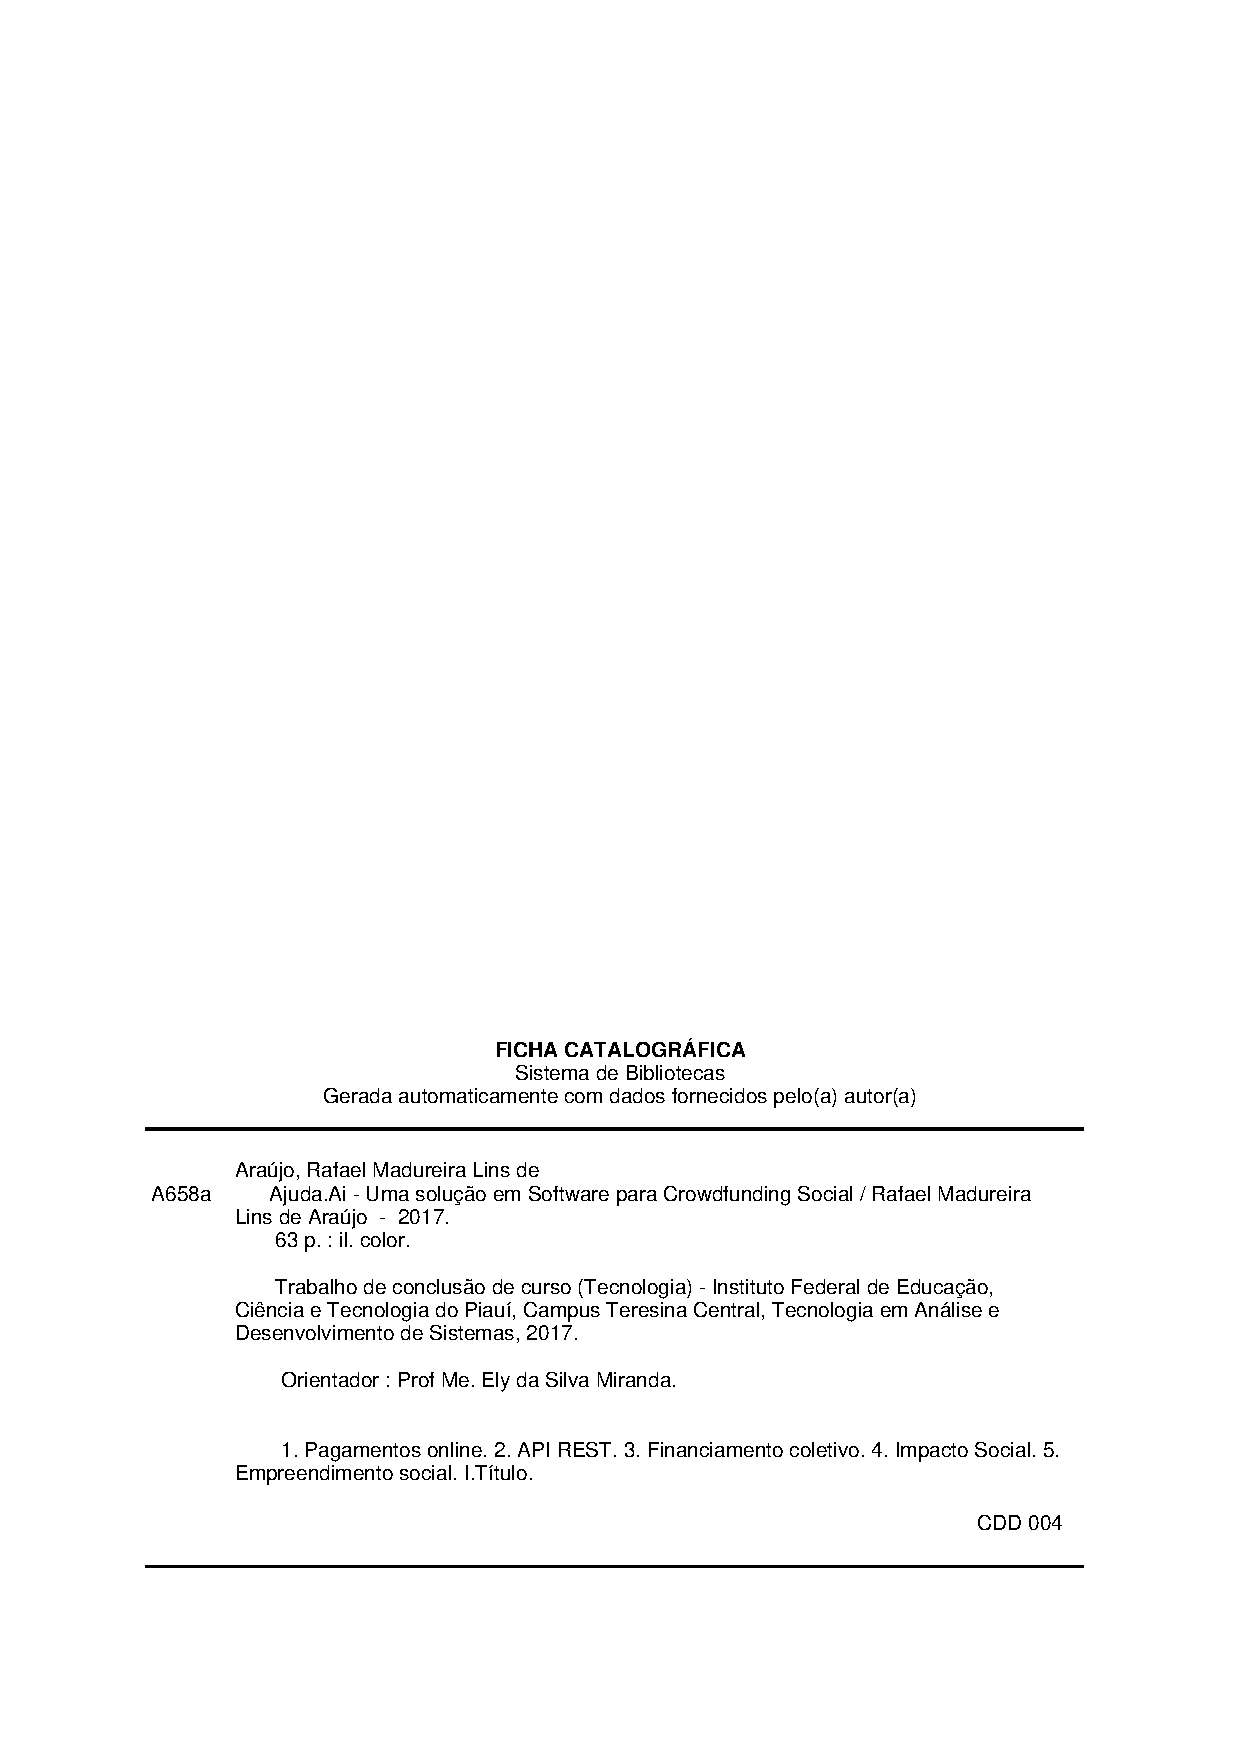
\includepdf{pre-textual/ficha-catalografica.pdf}

%% Caso queira fazer a ficha "tradicional" (este serve apenas como um modelo)
%\begin{fichacatalografica}
%	\sffamily
%	\vspace*{\fill}					% Posição vertical
%	\begin{center}					% Minipage Centralizado
%	\fbox{\begin{minipage}[c][8cm]{13.5cm}		% Largura
%	\small
%	\imprimirautor
%	
%	\hspace{0.5cm} \imprimirtitulo  / \imprimirautor. --
%	\imprimirlocal, \imprimirdata-
%	
%	\hspace{0.5cm} \thelastpage p. : il. (algumas color.) ; 30 cm.\\
%	
%	\hspace{0.5cm} \imprimirorientadorRotulo~\imprimirorientador\\
%	
%	\hspace{0.5cm}
%	\parbox[t]{\textwidth}{\imprimirtipotrabalho~--~\imprimirinstituicao,
%	\imprimirdata.}\\
%	
%	\hspace{0.5cm}
%		1. Palavra-chave1.
%		2. Palavra-chave2.
%		2. Palavra-chave3.
%		I. Orientador.
%		II. Universidade xxx.
%		III. Faculdade de xxx.
%		IV. Título 			
%	\end{minipage}}
%	\end{center}
%\end{fichacatalografica}


%% 03: Errata
%% Errata
%\begin{errata}
%Elemento opcional da norma ABNT NBR14724 de 2011. Exemplo:
%
%\vspace{\onelineskip}
%
%FERRIGNO, C. R. A. \textbf{Tratamento de neoplasias ósseas apendiculares com reimplantação de enxerto ósseo autólogo autoclavado %associado ao plasma rico em plaquetas}: estudo crítico na cirurgia de preservação de membro em cães. 2011. 128 f. Tese (Livre-Docência) %- Faculdade de Medicina Veterinária e Zootecnia, Universidade de São Paulo, São Paulo, 2011.

%% Tabela de exemplo com os erros
%\begin{table}[htb]
%\center
%\footnotesize
%\begin{tabular}{|p{1.4cm}|p{1cm}|p{3cm}|p{3cm}|}
%  \hline
%   \textbf{Folha} & \textbf{Linha}  & \textbf{Onde se lê}  & \textbf{Leia-se}  \\
%    \hline
%    1 & 10 & auto-conclavo & autoconclavo\\
%   \hline
%\end{tabular}
%\end{table}
%
%\end{errata}



%% 04: Folha de Aprovação
\imprimirfolhadeaprovacao
%% Use esta se forem 4 membros na banca:
%\imprimirfolhadeaprovacaoduascolunas



%% 05: Dedicatória
%%% Dedicatória do seu trabalho
%\begin{dedicatoria}
%	%% Empura o texto a seguir para a parte de baixo da página
%	\vspace*{\fill}
%    
%    %% Alinhado a Direita
%    \center
%    \begin{flushright}
%    	Dedico este trabalho à minha família.
%    \end{flushright}
%    
%    %% Descomente a linha seguir para deixar o texto centralizado verticalmente na página
%    %% Lembre de comentar o "\begin{}" e "\end{}" acima para centralizar o texto da dedicatória.
%	%\vspace*{\fill}
%%\end{dedicatoria}



%% 06: Agradecimentos
%% Agradecimentos
\begin{agradecimentos}
Agradeço aos meus pais, que me incentivaram e me apoiaram durante todo meu processo educacional e no meu dia-a-dia.  Aos meus familiares, que mesmo não estando próximos, sempre perguntavam como estavam meus estudos, minha vida.

Também agradeço todos os outros professores que passaram pela minha vida educacional, aos companheiros de trabalho, que sempre que precisava de alguma ajuda, estavam lá para me ajudar resolver o problema juntos. Não menos importante, agradeço aos meus amigos, os quais fizeram grande diferença na minha vida e que jamais serão esquecidos.

A todos que , independente da forma , fizeram parte da minha formação, o meu muito obrigado.

\end{agradecimentos}



%% 07: Epígrafe
%% Epígrafe
%% Uma frase que lhe inspira ou a qual lhe inspirou a fazer este trabalho
\begin{epigrafe}
\vspace*{\fill}
\begin{flushright}
\emph{"Não devemos nos questionar porque algumas coisas nos acontecem e sim o que podemos fazer com o tempo que nos é dado" 
\\ (Senhor dos Anéis – A Sociedade do Anel)}
\end{flushright}
\end{epigrafe}



%% 08: Resumo
%% Resumo
\begin{resumo}
As redes sociais tem como propósito o compartilhamento de conhecimentos e informações. Com a grande popularização da internet as redes sociais se virtualizaram, atendendo as necessidades de comunicação e os relacionamentos da vida real usando o ambiente virtual. Em paralelo a evolução da internet e das redes sociais, outra area que obteve grande crescimento foi o vegetarianismo e veganismo. Grande parte dos adeptos deste regime alimentar iniciam essa prática devido as questões relacionadas a saúde, economia, ambiente, ética e religião. Em busca de uma alimentação adequada, muitos seguidores optam em começar a fazer suas próprias refeições ao invés buscarem em restaurantes. O presente trabalho apresenta o desenvolvimento de um aplicativo mobile implementado na plataforma híbrida Ionic, que produz código executável para os ambientes operacionais IOS 7+ e Android 4.2+, além de integrada ao Facebook. O aplicativo irá funcionar como uma rede social, onde os usuários poderão publicar receitas, disponibilizá-las para todos que estiverem usando o aplicativo. Poderão curtir, favoritar e comentar na receita publicada como também seguir quem publicou a receita, criando assim, um vínculo social dentro do aplicativo.

\vspace{\onelineskip}
\noindent\\
\textbf{Palavras-chaves}: Redes sociais, vegetarianismo, veganismo, aplicativo mobile, Ionic, IOS, Android, Facebook.
\end{resumo}

%% 09: Abstract/Resumo em língua estrangeira
%% Abstract (configurado para língua inglesa)
\begin{resumo}[Abstract]			% Título do Resumo (Abstract = Resumo em inglês)
\begin{otherlanguage*}{english}		% Língua do texto
  The purpose of social networks is to share knowledge and information. With the great popularization of the Internet, social networks have become virtualized, meeting the needs of communication and real-life relationships using the virtual environment. In parallel to the evolution of the internet and social networks, another area that has grown enormously was vegetarianism and veganism. Many of the adherents of this diet begin this practice due to issues related to health, economy, environment, ethics and religion. In pursuit of adequate food, many followers choose to start making their own meals rather than going to restaurants. The present work presents the development of a mobile application implemented in the Ionic hybrid platform, which produces executable code for the IOS 7+ and Android 4.2+ operating environments, as well as integrated with Facebook. The application will act as a social network, where users can post recipes, make them available to everyone who is using the app. They can enjoy, favor and comment on the published recipe as well as follow who posted the recipe, thus creating a social bond within the application.
  
\vspace{\onelineskip}
\noindent\\
\textbf{Keywords}: Social networks, vegetarianism, veganism, mobile application, Ionic, IOS, Android, Facebook.
\end{otherlanguage*}
\end{resumo}

%% Exemplo de resumo em francês
%\begin{resumo}[Résumé]
% \begin{otherlanguage*}{french}
%    Il s'agit d'un résumé en français.
% 
%   \textbf{Mots-clés}: latex. abntex. publication de textes.
% \end{otherlanguage*}
%\end{resumo}

%% Exemplo de resumo em Espanhol
%\begin{resumo}[Resumen]
% \begin{otherlanguage*}{spanish}
%   Este es el resumen en español.
%  
%   \textbf{Palabras clave}: latex. abntex. publicación de textos.
% \end{otherlanguage*}
%\end{resumo}
% ---



%% 10: Lista de Ilustrações
%% Lista de Ilustrações
\pdfbookmark[0]{\listfigurename}{lof}
\listoffigures*
\cleardoublepage



%% 11: Lista de Tabelas
%% Lista de Tabelas
\pdfbookmark[0]{\listtablename}{lot}
\listoftables*
\cleardoublepage





%% 12: Lista de Abreviaturas e Siglas
%%% Lista de Siglas
\begin{siglas}
  \item[CDN] CONTENT DELIVERY NETWORK
  \item[CSS] CASCADING STYLE SHEETS
  \item[HTTP] HYPERTEXT TRANSFER PROTOCOL 
  \item[HTML] HYPERTEXT MARKUP LANGUAGE 
  \item[IDE] INTEGRATED DEVELOPMENT ENVIRONMENT 
  \item[IP] INTERNET PROTOCOL 
  \item[PEP] PYTHON ENHANCEMENT PROPOSAL 
  \item[P2P] PEER TO PEER
  \item[RSS] REALLY SIMPLE SYNDICATION
  \item[WSGI] WEB SERVER GATEWAY INTERFACE
  \item[WWW] WORLD WIDE WEB 
  \item[ARPA] ADVANCED RESEARCH PROJECT AGENCY
  \item[ORM] OBJECT-RELATIONAL MAPPING
\end{siglas}



%% 13: Lista de Símbolos
%%% Lista de Símbolos
%% (esta é apenas uma lista de exemplo)
%\begin{simbolos}
%  \item[$ \Gamma $] Letra grega Gama
%  \item[$ \Lambda $] Lambda
%  \item[$ \zeta $] Letra grega minúscula zeta
%  \item[$ \in $] Pertence
%\end{simbolos}



%% 14: Sumário (o asterisco retira o próprio sumário do sumário)
\pdfbookmark[0]{\contentsname}{toc}
\tableofcontents*
\cleardoublepage


%% Indica que a partir daqui ficarão os elementos textuais (TCC em si)
\textual

%% Inclui os capítulos do TCC (parte textual)
%% %%%%%%%%%%%%%%%%%%%%%%%%%%%%%%%%%%% %%
%% Elementos Textuais (Capítulos)      %%
%% %%%%%%%%%%%%%%%%%%%%%%%%%%%%%%%%%%% %%

%% Inclua aqui os capítulos que farão parte do TCC
% ----------------------------------------------------------
% Introdução
% ----------------------------------------------------------

\chapter{Introdução}

Neste capítulo introdutório será feita uma contextualização sobre a evolução da internet, impactos e crescimento tanto das redes sociais quanto vegetarianismo e veganismo, juntamente com a apresentação das justificativas que levaram ao desenvolvimento do aplicativo para dispositivos móveis proposto neste trabalho.

\section{Contextualização}

A Internet nasceu da soma de pequenas conquistas tecnológicas com o passar dos anos. No inicio da década de 90, desde que foi aberta comercialmente, a internet tem passado por grandes mudanças, evoluindo cada vez mais, criando milhares de recursos e possibilidades de facilitar e organizar conteúdos e informações dos mais diversos tipos. É perceptível as enormes transformações que a internet vem causando nas comunicações, no trabalho, no comércio, no entretenimento.

Inicialmente os \textit{sites} surgiram praticamente para o compartilhamento de informações, de uma forma simples e direta, apenas com textos. Anos depois com mais tecnologias disponíveis, os \textit{sites} ja eram mais trabalhados, com mais detalhes em seu \textit{layout}, tendo imagens e cores. Em constante evolução a internet continuou agregando cada vez mais novas funcionalidades, dando espaço para usar novas tecnologias para deixar os sites com mais conteúdos e mais atraentes.

Com o surgimento da Web 2.0, em meados dos anos 2000, que visava atender às necessidades das novas gerações, tornando a internet mais dinâmica, livre e colaborativa, um outro tipo de serviço de comunicação e entretenimento começou a ganhar força: as redes sociais. Rede social significa interação e troca social, compartilhando interesses e conhecimento. O ser humano por natureza sempre busca se comunicar, segundo \citeauthor{oliveira-marta}, “é a necessidade de comunicação que impulsiona, inicialmente, o desenvolvimento da linguagem”.

As redes sociais mudaram a forma como as pessoas avaliam o que acontece ao seu redor. Segundo \citeauthor{patricio-utilizacao}, as redes sociais são aplicações que suportam um espaço comum de interesses, necessidades e metas comuns para a colaboração, partilha de conhecimento, interação e comunicação. Além disso, são excelentes ferramentas que podem ser usadas para promover o pensamento crítico e fornecer oportunidades de debates.

No entanto, as pessoas tendem a ficar cansadas de utilizar o mesmo serviço todos os dias e iniciam uma busca por algo novo. Com isso, surgem as redes sociais de nicho, que estão tendo um destaque cada vez maior na internet. As pessoas estão interessadas em assuntos comuns, e não pretendem abranger um grande número de usuários. 

A procura se deve porque o usuário quer algo mais específico de acordo com suas preferências e não um ambiente em que se fala de tudo, até do que não o agrada. É o caso das pessoas adeptas ao vegetarianismo. É cada vez mais comum, nos círculos de amigos e/ou familiares e nas redes sociais, encontrar pessoas que optaram pelo estilo de vida natural. A busca pela qualidade de vida, compaixão e respeito pelos animais são alguns dos motivos que têm colaborado com o crescimento do vegetarianismo.

No entanto, mesmo com a crescente adesão ao vegetarianismo, nota-se uma grande dificuldade em encontrar produtos de boa procedência, restaurantes, entre outros estabelecimentos. Até mesmo quando se encontrado locais que os vegeterianos possam vir se alimentar, o cardapio se torna limitado, com poucas opções e nem sempre agradam. Diante desses empecilhos, a melhor solução é sempre fazer sua própria alimentação, buscando os diversos tipos e variados de receita vegetarianas e veganas.

Nesse contexto, aplicativos para o nicho vegetariano foram surgindo. Atualmente,  existem alguns aplicativos de receitas culinárias voltado para o vegetarianismo, mas não possuem um foco social, apenas informações já cadastradas para que os usuários possam usufruir, mas sem ter um vinculo social com outros usuários, o que é importante pela necessidade de colaboração, partilha de conhecimento, interação e comunicação.

Tendo em vista as informações apuradas sobre redes sociais, dispositivos móveis , vegetarianismo e veganismos, consideramos neste trabalho o desenvolvimento de uma aplicativo móvel, que permite os usuários disponibilizarem no ambiente virtual seus interesses pessoais e/ou conhecimentos por receitas culinárias vegetarianas, sendo possível o detalhamento completo de uma receita culinária vegetariana e / ou vegana, contendo a inserção de imagens e outras informações pertinentes, de modo a deixá-la simples e de fácil entendimento. Foi realizada uma pesquisa nas principais lojas virtuais, tais como Google Play e Apple Store , onde foram encontrados algumas aplicações voltadas ao nicho vegetariano, mas nenhuma com o intuito social que o presente trabalho venha a apresentar. Veja na tabela abaixo:

\begin{table}[H]
	\centering
	\caption{Alguns aplicativos nas lojas virtuais voltado para o nicho vegetariano e vegano.}
	\label{tabela-aplicativos-vegetarianos-veganos}
	\begin{tabular}{|l|c|c|l|}
	\hline
	\textbf{} & \textbf{Google Play} & \textbf{Apple Store} & \textbf{Descrição} \\ \hline
	21 – Day Vegan Kickstar & - & x & \begin{tabular}[c]{@{}l@{}}Propõe refeições completas \\ por 21 dias\end{tabular} \\ \hline
	I`m Hungry & x & - & \begin{tabular}[c]{@{}l@{}}Contém diversas receitas \\ pré cadastradas\end{tabular} \\ \hline
	Vgan & x & - & \begin{tabular}[c]{@{}l@{}}Seu foco principal são \\ informações sobre bebidas\end{tabular} \\ \hline
	BeVeg & x & x & \begin{tabular}[c]{@{}l@{}}Delivery de restaurante\end{tabular} \\ \hline
	HappyCow & x & x & \begin{tabular}[c]{@{}l@{}}Um guia onde indica \\ restaurantes, bares e lojas\end{tabular} \\ \hline
	\end{tabular}
\end{table}

É importante ressaltar que, como o ambiente da aplicação é uma rede social , essas informações serão compartilhadas por todos os usuários da rede, por meio de uma timeline ou linha do tempo, na qual poderão ver todas as publicações de todos os demais usuários adicionados na sua rede. 

\section{Justificativa}

De acordo com um relatório realizado pelo \citeauthor{eMarketer}, em 2017 pelo menos 71\% dos internautas em todo o mundo terão acesso a redes sociais, como pode ser visto por meio da  Figura \ref{fig:figura1}.

\begin{figure}[H]
	\caption{\label{fig:figura1}Usuários de rede social e penetração em todo o mundo.}
	\centering
	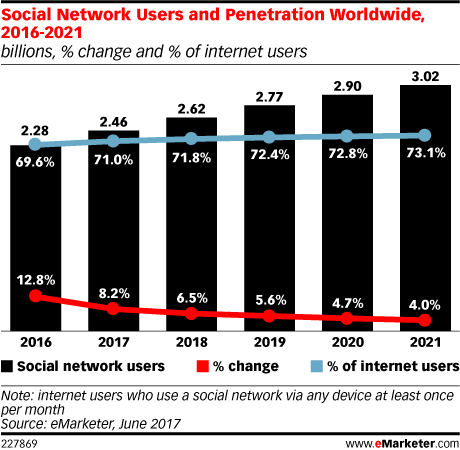
\includegraphics[scale=0.5]{imagens/figura1.png}
	\legend{Fonte: \citeauthor{eMarketer}}
\end{figure}

Com a expansão das redes sociais, o uso de dispositivos móveis vem crescendo consideravelmente no mundo. Em 2014 o acesso à internet por meio de dispositivos móveis superou o acesso por meio de desktops, como pode ser visto na Figura \ref{fig:figura2}.

\begin{figure}[H]
	\caption{\label{fig:figura2}Projeção Global de usuários de desktop vs. usuários de internet móvel.}
	\centering
	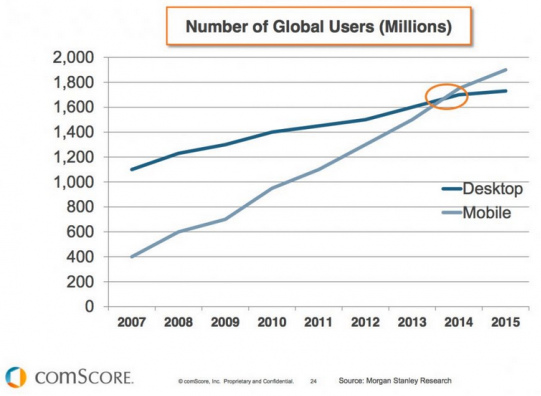
\includegraphics[scale=0.5]{imagens/figura2.png}
	\legend{Fonte: \citeauthor{smartinsights}}
\end{figure}

A \citeauthor{svb} - Sociedade Vegetariana Brasileira, divulgou uma pesquisa realizada pelo Instituto Brasileiro de Opinião Pública e Estatística, IBOPE, que 15,2 milhões de brasileiros se declaram vegetarianos, isso corresponde a 8\% da população do país. De acordo com o Google Trends, de Janeiro de 2012 a Julho de 2016 o volume de buscas pelo termo ‘vegano’ cresceu 1000\% (mil por cento) no Brasil.

Assim, existe uma necessidade preemente de mobile + redes sociais + veganismo/vegetarianismo, surgindo a ideia da criação de um aplicativo envolvendo essas três conceitos.
 
\section{Objetivos}

Nesta seção serão apresentados o objetivo geral e os específicos do presente trabalho.

\subsection{Objetivo Geral}

Desenvolver uma rede social de receitas culinárias vegetarianas e veganas, implementada em uma ferramenta tecnológica híbrida , que poderá funcionar nos sistemas operacionais mais utilizados atualmente: Android e IOS.

\subsection{Objetivos Específicos}
\begin{lista}
  \item Apresentar o referencial teórico sobre as tecnologias a serem utilizadas;
  \item Desenvolver análise e projeto do sistema proposto como estudo de caso;
  \item Codificar o aplicativo utilizando técnicas apropriadas através o framework Ionic;
  \item Realizar teste de usabilidade da interface criada, para que possa ter um resultado satisfatório e eficaz;
  \item Disponibilizar para o usuário uma versão do aplicativo para download (Google Play).
\end{lista}
% ----------------------------------------------------------
% Fundamentação Teórica
% ----------------------------------------------------------
\chapter{Fundamentação Teórica} \label{cha:fundamentacao}

Neste capítulo serão apresentados os conceitos teóricos utilizados como base para a proposição e desenvolvimento deste trabalho.

\section{Dispositivos móveis e aplicativos híbridos}

Segundo \citeauthor{b2005mobile}, sistemas computacionais móveis são sistemas que podem facilmente ser movidos fisicamente ou cujas capacidades podem ser utilizadas enquanto eles estão sendo movidos. Como estes sistemas preveem tal mobilidade, terminam por oferecer recursos e características que não encontramos em sistemas comuns, como por exemplo: preocupação com nível de energia, armazenamento de dados local/remoto e comunicação com outros sistemas.

Os sistemas computacionais móveis, são desenvolvidos para rodar em celulares, tablets e similares. Para um entendimento mais simples: dispositivo ou sistema móvel deve oferecer a possibilidade de acesso imediato e com o usuário em movimento.

De acordo com um artigo publicado pelo \citeauthor{firstmobile}, a ideia de lançar o primeiro telefone móvel surgiu em 1947 quando um grupo de pesquisadores resolveu melhorar a forma de comunicação a distância. Como naquela época não havia tecnologia suficiente,  essa ideia só saiu do papel em 1973 quando a Motorola, empresa de telecomunicações multinacional americana, apresentou o primeiro aparelho realmente móvel e portátil, DynaTAC 8000X. 

Dos anos 90 para os dias atuais muita coisa mudou numa  velocidade muitíssimo rápida. As tecnologias de transmissão evoluíram e passaram a ser digitais, os equipamentos ficaram menores e muito mais eficientes. Os dispositivos móveis tornaram-se uma ferramenta tão eficiente que deixaram de ser utilizados apenas para ligações e envio de mensagem de texto, se tornando parte integrante da vida moderna em todo o mundo, como pode ser visto na Figura \ref{fig:figura3} 

\begin{figure}[H]
	\caption{\label{fig:figura3}Usuários de dispositivos móveis em todo mundo}
	\centering
	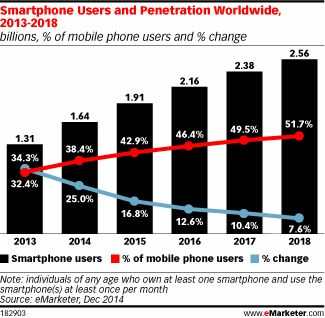
\includegraphics[scale=0.5]{imagens/figura3.jpg}
	\legend{Fonte: \citeauthor{eMarketer}}
\end{figure}

Os dispositivos móveis funcionam juntamente com um sistema operacional. Esse sistema é a plataforma de interação entre o usuário e o dispositivo, onde todos os seus aplicativos serão armazenados e irão funcionar. Hoje, no mercado, há alguns sistemas que se destacam pela qualidade e popularidade, os mais conhecidos são: Android do Google (93,2\% no Brasil e 55,3\% nos Estados Unidos) e IOS da Apple (6,3\% no Brasil e 43,9\% nos Estados Unidos), números baseados numa pesquisa feita pela empresa de analise de dados \citeauthor{kantar}, realizada em 2017. As companhias de tecnologia que desenvolvem os sistemas operacionais disponibilizam Kits de Desenvolvimento de Software (SDK) que permitem aos desenvolvedores criarem e comercializarem milhares de aplicativos com as mais inúmeras funcionalidades em suas lojas virtuais. 

Cada sistema operacional possui a sua própria arquitetura, o que exige o desenvolvimento de aplicações com tecnologias nativas que consigam explorar os seus potenciais específicos. Normalmente, isso implica em linguagens de programação, ferramentas e processos de distribuição específicos (mas não restritos) daquela plataforma. Para um aplicativo nativo do sistema operacional IOS, por exemplo, você precisaria utilizar um Mac, XCode como IDE e desenvolveria em Objetive-C ou Swift.  Por sua vez, um aparelho que tenha como sistema operacional Android poderia ser mais flexível quanto ao computador, mas provavelmente usaria Java como linguagem e o Android Studio como IDE. A Figura \ref{fig:figura4} mostra um pouco essa diferença.

\begin{figure}[H]
	\caption{\label{fig:figura4}Conceito da junção do aplicativo nativo com a aplicação web.}
	\centering
	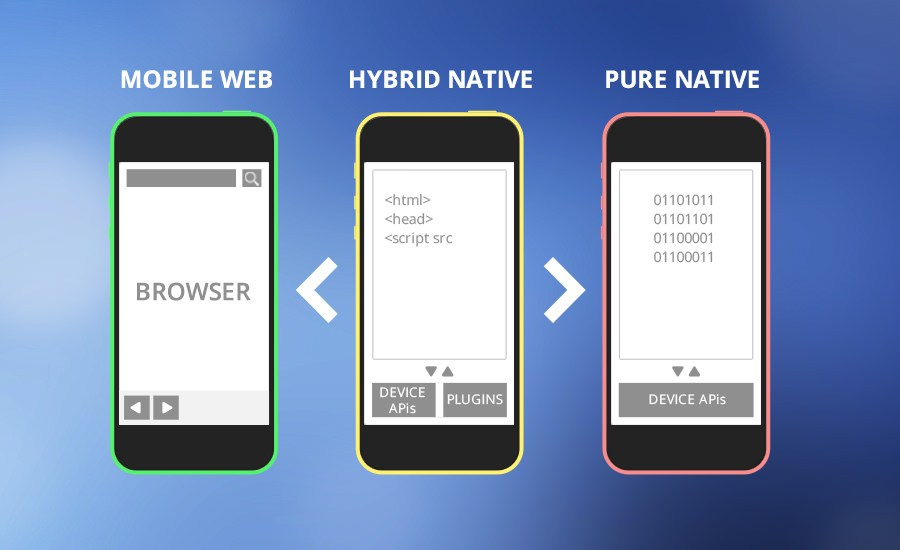
\includegraphics[scale=0.5]{imagens/figura4.jpg}
	\legend{Fonte: Google images}
\end{figure}

Webview é um componente nativo dos sistemas operacionais, que é executado assim que o aplicativo é aberto pelo usuário e contém apenas o necessário para que o aplicativo em HTML5, CSS e JavaScript funcione, se comportando como um motor de renderização do aplicativo, permitindo que tenhamos muito mais recursos do que uma simples página web. 

O desenvolvimento de um aplicativo híbrido acaba sendo mais rápido e também mais barato. A redução de tempo em comparação aos aplicativos nativos se deve à possibilidade de execução do aplicativo híbrido em diferentes plataformas. Devido a essa característica, não há a necessidade de desenvolver o aplicativo várias vezes para se adequar a distintas plataformas, gerando menos impacto sobre o orçamento. Muitas empresas também optam pelo desenvolvimento de aplicativo híbrido em situações que não exigem uma alta performance do aplicativo ou quando o público-alvo é heterogêneo. Nesses casos, uma solução mais genérica para ser usada em plataformas variadas se torna mais vantajosa. A tabela 2 mostra um comparativo entre aplicativos híbridos e nativos.

\begin{table}[H]
	\centering
	\caption{Comparativo entre aplicativos híbridos e nativos.}
	\label{tabela-comparativo-aplicativos-hibridos-nativos}
	\begin{tabular}{|l|c|c|c|}
	\hline
	\textbf{} & \textbf{Híbridos} & \textbf{Nativo (Android / Ios)} & \textbf{Melhor} \\ \hline
	Gráfico & HTML, Canvas, SVG & APIs Nativas & \begin{tabular}[c]{@{}l@{}} Nativo\end{tabular} \\ \hline
	Performance & Lenta & Rápida & \begin{tabular}[c]{@{}l@{}} Nativo\end{tabular} \\ \hline
	Aparência & Emulado & Aparência real & \begin{tabular}[c]{@{}l@{}} Nativo\end{tabular} \\ \hline
	Recursos do equipamento & Muita & Total & \begin{tabular}[c]{@{}l@{}} Nativo\end{tabular} \\ \hline
	Publicação nas lojas & Quase normal & Normal & \begin{tabular}[c]{@{}l@{}} Híbrido\end{tabular} \\ \hline
	Reutilização do código & Total & Nenhuma & \begin{tabular}[c]{@{}l@{}} Híbrido\end{tabular} \\ \hline
	Custo de desenvolvimento & Médio & Alto & \begin{tabular}[c]{@{}l@{}} Híbrido\end{tabular} \\ \hline
	Tempo de desenvolvimento & Baixo & Alto & \begin{tabular}[c]{@{}l@{}} Híbrido\end{tabular} \\ \hline
	Facilidade de atualização & Fácil & Médio & \begin{tabular}[c]{@{}l@{}} Híbrido\end{tabular} \\ \hline
	Conhecimentos requeridos & HTML5, CSS e Javascript & Java, ObjectiveC e Swift & \begin{tabular}[c]{@{}l@{}} Híbrido\end{tabular} \\ \hline
	Curva de aprendizado & Média & Lenta & \begin{tabular}[c]{@{}l@{}} Híbrido\end{tabular} \\ \hline
	
	\end{tabular}
\end{table}


\section{Redes sociais}

Os seres humanos são sociais por natureza, vivem em comunidades, rodeados por outras pessoas. O compartilhamento de informações e interesses entre elas mesmas, são características marcantes da rede social, conhecimentos dos mais diversos tipos, instigam as pessoas a partilhar essas informações e irem a procura de novos conceitos e ideias.

As pessoas estão inseridas em uma sociedade com base nos relacionamentos que desenvolvem durante toda a vida. Estes relacionamentos partilham conhecimento e interesses em comum. As redes sociais são compostas por pessoas (ou organizações) conectadas através destes laços sociais \citeauthor{watts2003}. Com à internet, as redes sociais vêm conquistando cada vez mais adeptos, reunindo pessoas com os mais diversos objetivos e possibilitando a ampliação da sua rede de  relacionamento com pessoas conhecidas ou não, dos mais diversos tipo e lugares, aumentando ainda mais e facilitando a aquisição e compartilhamento de novidades. Como em todo grupo social, existem padrões de comportamento e naturalmente, todas as atitudes consideradas ruins pela comunidade excluem os usuários que o fazem e as atitudes consideradas boas trazem retorno positivo, como uma espécie de recompensa. É importante também que haja um esforço para tentar evitar que usuários e conteúdos falsos sejam criados, para que a credibilidade em geral não seja perdida. Com base nesses conceitos, as redes sociais foram potencializadas através de aplicações web e aplicativos móveis que facilitaram a integração dos seus usuários e estão em crescente uso e expansão, oferecendo diferentes tipos de serviço dependendo das necessidades e preferências dos usuários. Existem redes para fazer negócios, fazer contato com amigos e familiares, conhecer novas pessoas, compartilhar informações. 

Cada uma das redes sociais tem um objetivo, forma e conteúdo diferentes. A sociedade precisa entender e adaptar-se a cada uma delas, buscar ter uma conteúdo que esteja de acordo com a essência de cada uma. Hoje,  as possibilidades são imensas: blogs, locais  de compartilhar musicas, vídeos, de pesquisa, consulta. Na Figura \ref{fig:figura5}, mostramos as principais redes sociais com os seus respectivos números de usuários: 

\begin{figure}[H]
	\caption{\label{fig:figura5}Principais redes sociais com seus respectivos usuários.}
	\centering
	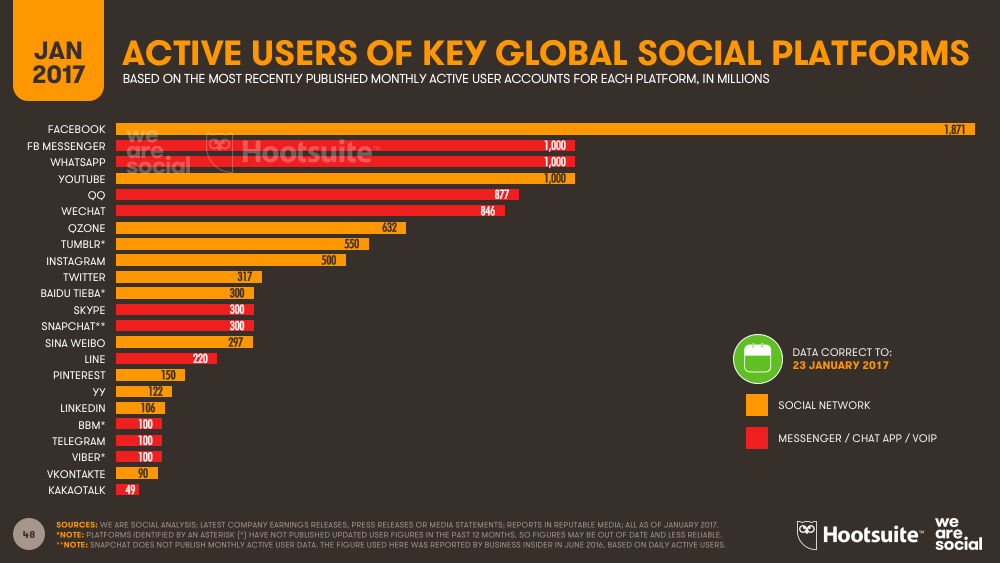
\includegraphics[scale=0.5]{imagens/figura5.png}
	\legend{Fonte: \citeauthor{wearesocial}}
\end{figure}

Baseado na quantidade de usuários utilizando as mais diversas redes sociais, é possível perceber a grande penetração da internet na população mundial e consequentemente podemos observar o grande poder que as redes sociais possuem. Tendo isso em vista, as empresas de diversas áreas acabam investindo cada vez mais nesse mercado que só cresce. Dependendo do público e alcance, investir nas redes sociais acaba sendo uma maneira rápida, fácil e barata de conquistar espaço nesse mercado.

No Brasil, varias empresas estão presentes em pelo menos uma rede social. A presença nas redes sociais acaba sendo um facilitador em entrar em contato com seu publico podendo assim atender as necessidades dos mesmos com uma maior facilidade, aumentando a divulgação dos seus produtos e conquistando novos usuários.

\section{Vegetarianismo}

O vegetarianismo surgiu há cerca de 5 milhões de anos atrás. O
antepassado mais antigo do homem, o Australopithecus Anamensis, alimentava-se
somente de frutas, folhas e sementes, vivendo em perfeita harmonia com os
menores animais, que poderia facilmente apanhar para se alimentar. O domínio do
fogo e o desenvolvimento das armas vêm mudar essa realidade, onde o Homo
Neanderthalensis, caçava, em grupos de 10 a 15, animais de grande porte como os
mamutes e outros de pequeno porte como os veados, dos quais tudo era
meticulosamente aproveitado. Mais tarde, as populações humanas foram criando
culturas de vegetais fixas, que começaram a atrair animais como porcos selvagens,
ovelhas, cães, cabras, aves, ratos e pequenos felinos, que foram sendo
domesticados. Alguns animais começaram a ser mortos para consumo. Foi então
que o homem se tornou sedentário e começou a encarar os animais como alimentos
(\citeauthor{rodrigues2005}, 2005).


Segundo \citeauthor{couceiro2008}(2008, p.365), para que se entenda a origem do vegetarianismo, diz que “o vegetarianismo tem suas origens desde os primórdios da criação do homem e um de seus registros mais amplamente reconhecidos é encontrado no Velho Testamento, na passagem em que Deus diz a Adão e Eva qual deveria ser seu alimento. “

O vegetarianismo tem como premissa a prática de comer alimentos derivados das plantas e não usufruindo de alimentos derivados de origem animal. Com a crescimento do conhecimento e informações sobre os benefícios dos vegetais à saúde, as pessoas passaram a ver a dieta vegetariana como uma melhoria da qualidade de vida. A tabela 3, mostra os países com as maiores taxas de vegetarianismo.


\begin{table}[H]
	\centering
	\caption{Países com as mais altas taxas de vegetarianismo}
	\label{paises-com-as-mais-altas-taxas-de-vegetarianimos}
	\begin{tabular}{|c|c|c|}
	\hline
	\textbf{Classificação} & \textbf{Países com as mais altas taxas de vegetarianismo} & \textbf{Prevalência} \\ \hline
	1  & Índia & 38\% \\ \hline
	2  & Israel & 13\% \\ \hline
	3  & Taiwan & 12\% \\ \hline
	4  & Itália & 10\% \\ \hline
	5  & Áustria & 9\% \\ \hline
	6  & Alemanha & 9\% \\ \hline
	7  & Reino Unido & 9\% \\ \hline
	8  & Brasil & 8\% \\ \hline
	9  & Irlanda & 6\% \\ \hline
	10 & Austrália & 5\% \\ \hline
	\end{tabular}
\end{table}

Segundo \citeauthor{worldatlas2017}, as influências religiosas e culturais contribuem para os altos níveis de vegetarianismo da Índia em relação às normas globais. No caso de Israel, apenas 13\% do seu povo é formado por vegetarianos, influenciados por princípios relacionados com a religião. Os judeus tradicionais obedecem às leis dietéticas kashrut que defendem que um intervalo de seis horas deve ser mantido entre o consumo de leite e carne. Em Taiwan, 12\% da população são vegetarianos, influenciados pela culinárias, religiosidade e fatores governamentais. No caso da Itália tem a maior percentagem de vegetarianos encontrados na União Europeia. A Áustria, Reino Unido e Alemanha contam 9\% de sua população como vegetarianos, ambos com influências sociais e culinárias, apesar de que a Alemanha tem sua reputação como um país amante da carne.  No Brasil, 8\% da população é vegetariana, as influências culinárias e econômicas podem ter sido um fator no vegetarianismo no Brasil. A Irlanda conta com cerca de 6\% de vegetarianos em relação à população total. 5\% dos australianos seguem uma dieta vegetariana.

De uma forma genérica, o vegetarianismo é um regime alimentar que exclui da dieta todos os tipos de carne, bem como todos alimentos derivados. É baseado fundamentalmente no consumo de alimento de origem vegetal, com ou sem o consumo de laticínios e/ou ovos. Ovos e laticínios, embora sejam de origem animal, estão incluídos na dieta de alguns vegetarianos. Por essa e outras diferenças, que os vegetarianos são sendo categorizados em 4 grupos principais citados na Figura \ref{fig:figura6}.

\begin{figure}[H]
	\caption{\label{fig:figura6}Tipos de vegetarianos.}
	\centering
	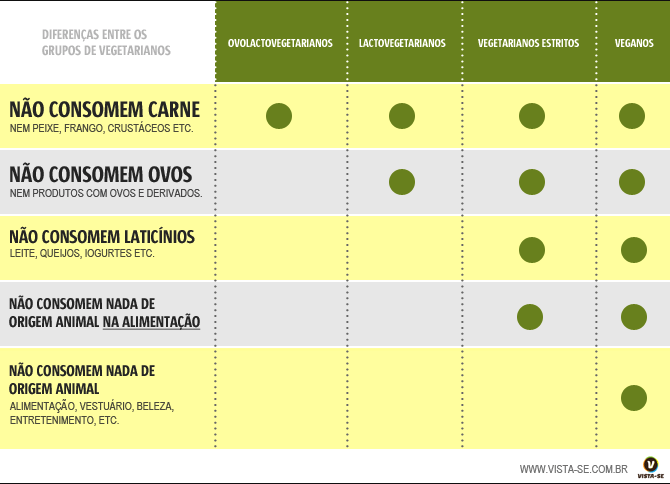
\includegraphics[scale=0.5]{imagens/figura6.png}
	\legend{Fonte: \citeauthor{tiposveggies}}
\end{figure}

Nas redes sociais, o vegetarianismo e veganismo tem ganho cada vez mais popularidade. Apesar de terem muitas semelhanças, ambos tem algumas diferenças, criando uma identidade completamente diferentes para os indivíduos que fazem parte destes grupos. Enquanto o vegetarianismo tem por sua base a alimentação, em não consumir nada de origem animal e derivados, o veganismo tem uma premissa mais ética, a luta pela libertação e não exploração animal, além da alimentação, os veganos não usufruem de nada de origem animal, incluindo roupas, cosméticos e remédios. Por isso os veganos estão sempre atentos sobre as empresas que fazem produtos e/ou testes em animais, buscando outras alternativas 

De acordo com aqueles que adotam a postura vegana, os animais não devem ser mortos e nem explorados para atender às nossas necessidades. A prática do veganismo vem carregada de sacrifícios e vontades negadas. 
% ----------------------------------------------------------
% Metodologia
% ----------------------------------------------------------
\chapter{Metodologia} \label{sec:metodologia}

Este capítulo descreve os materiais e métodos utilizados no desenvolvimento do aplicativo. 

\section{Metodologia de desenvolvimento} \label{sec:metodologia de desenvolvimento} 

No desenvolvimento do presente trabalho, foram utilizados os princípios das metodologias ágeis que têm como objetivo acelerar, adaptar e visar o melhor processo para o desenvolvimento do software, entregando o produto final  ao cliente com o que realmente deseja e com qualidade. Dentre dos modelos de processos ágeis, foi abordado o modelo de desenvolvimento de software enxuto.

O Desenvolvimento de Software Enxuto ou \textit{Lean Software Development} (LSD),
de acordo com \citeauthor{poppendiek2003}, é a aplicação dos princípios da \textit{Toyota Product Development System}  para o desenvolvimento de software que, quando aplicado de forma correta, possibilita alta qualidade, rapidez e baixo custo. Para atingir esse objetivo, o modelo de desenvolvimento Lean possui alguns princípios, Figura \ref{fig:principios-lean}. 


\begin{figure}[H]
	\caption{\label{fig:principios-lean}Princípios do modelo Lean}
	\centering
	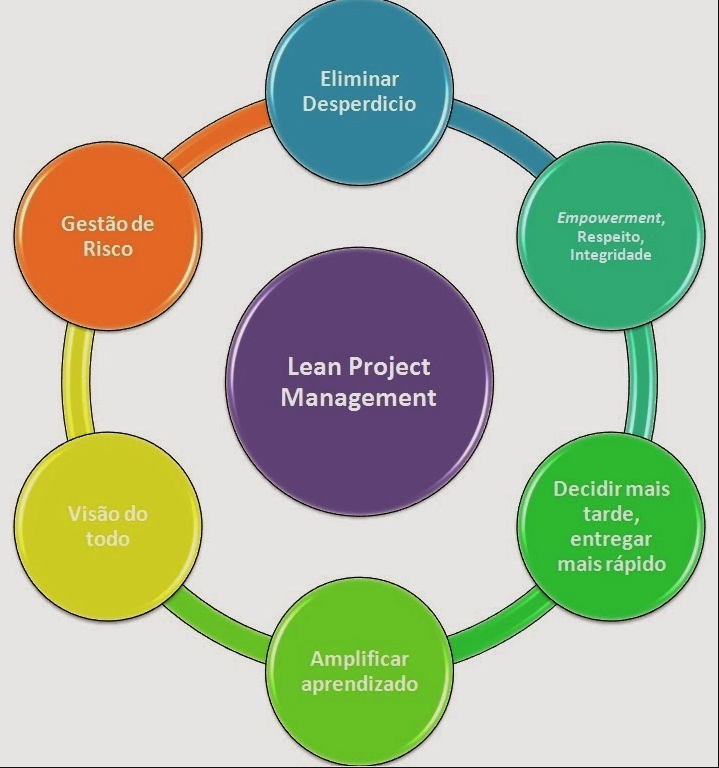
\includegraphics[scale=0.3]{imagens/figura7.png}
	\legend{Fonte: \citeauthor{rosamilha2014}}
\end{figure}

\section{Ferramentas e tecnologias utilizadas} \label{sec:ferramentas} 
Nesta seção, iremos apresentar alguns dos materiais que foram necessários para o desenvolvimento deste trabalho.


\subsection{Ionic Framework}

Ionic é uma combinação de tecnologias e utilitários projetados para tornar a construção de aplicativos móveis híbridos de forma rápida, fácil e bonita. Ele foi criado pela DriftyCo em 2012 e consiste em uma compilação de várias ferramentas que possibilitam o desenvolvimento de aplicações utilizando tecnologias e linguagens de programação web como HTML, CSS e Javascript.

Através do \citeauthor{ionic2017} Framework é possível desenvolver aplicações móveis híbridas com interface e a utilização de recursos das três plataformas mais utilizadas: Android, IOS e Windows Phone. Esse Framework também possibilita o desenvolvedor criar aplicações progressivas, que são websites móveis que possuem performance próxima da performance de um aplicativo nativo.

\subsection{Angular JS}
\citeauthor{angularjs2017} é um framework SPA (\textit{Single Page Applications}) em Javascript, de código aberto e mantido pelo Google,
que permite escrever aplicativos Web. Ele permite que você use HTML como sua linguagem de modelo e permite expandir a sintaxe do HTML para expressar os componentes da sua aplicação de forma clara e sucinta. A ligação de dados e a injeção de dependência da AngularJS eliminam muito do código que de outra forma você teria que escrever.

O Angular JS disponibiliza recursos completos para facilitar a criação de um aplicativo CRUD: 
\begin{lista}
	\item Vinculação de dados;
	\item Diretrizes básicas de modelos;
	\item Validação de formulários; 
	\item Roteamento;
	\item Componentes reutilizáveis;
	\item Injeção de dependência.
\end{lista}

\subsection{Ruby}

\citeauthor{ruby2017} é uma linguagem orientada a objetos, com tipagem forte e dinâmica criada por Yukihiro "Matz" Matsumoto, que misturou partes de suas linguagens favoritas (Perl, Smalltalk, Eiffel, Ada e Lisp) para formar uma nova linguagem com objetivo de ser uma linguagem simples de ler e ser entendida, para facilitar o desenvolvimento e manutenção de sistemas escritos com ela. Possui vários repositórios de bibliotecas disponíveis em sites como \textit{Ruby Forge} e \textit{Ruby Application Archive} (RAA). Existe, ainda, uma ferramenta bastante útil para instalação de bibliotecas, chamada \textit{Ruby Gems}. O software mais conhecido desenvolvido em Ruby é o \citeauthor{rubyonrails}.

\subsection{Facebook SDK}

O \citeauthor{facebooksdk} (Software Development Kit) está inserido em uma plataforma: a \textit{Facebook Platform}. Essa plataforma permite que qualquer um construa aplicativos sociais no Facebook e na Web, disponibilizando uma coleção abrangente de APIs e SDKs.

A principal API (\textit{Application Program Interface}) do Facebook Platform é API \textit{Graph}, que permite aos desenvolvedores criarem seus próprios aplicativos. Através desta API as aplicações podem acessar e reunir informações sobre o usuário (desde que o usuário tenha permitido o acesso as suas informações). 

A classe principal do Facebook SDK encapsula métodos que permitem autorizar o usuário, criar diálogos do Facebook, fazer solicitações de API, desconectar o usuário e ter ou definir informações de acesso e sessão, além do status. Quando os usuários acessam a aplicação,  poderão conceder permissões para que o aplicativo possa recuperar informações ou executar alguma ação no Facebook, no nome do usuário.


% ----------------------------------------------------------
% Vegood
% ----------------------------------------------------------
\chapter{Vegood} \label{cha:vegood}
Neste capítulo, apresentamos a aplicação Vegood, objeto deste trabalho. É sistema de arquitetura simples para dispositivos móveis, desenvolvido por meio de uma plataforma hibrida de forma a poder ser usado nas plataformas IOS 7+ e Android 4.2+, além  de integrada ao Facebook.

\section{Definição do produto} \label{sec:vegood:definicao}

O Vegood apresenta aos usuários uma rede social cuja temática é a culinária vegetariana e vegana, onde os usuários poderão publicar e disponibilizar receitas , além de  curtir , favoritar e comentar em receitas publicadas.

A aplicação possui duas formas de autenticação: uma através do próprio cadastro que poderá ser realizado no aplicativo, onde haverá uma tela de cadastro de usuário que preenche um formulário com os dados necessários para que uma conta seja criada; e uma outra, através do Facebook,  quando o usuário autoriza que a aplicação utilize as suas credenciais desta rede social para se logar. Após a autenticação o aplicativo abrirá sua tela principal.

O usuário também pode seguir e ser seguido por todos os usuários, assim criando um vínculo social dentro da aplicação. Além das funcionalidades já citadas, o Vegood também irá disponibilizar informações, dicas e mitos sobre o vegetarianismo. 

É importante ressaltar que a utilização plena da aplicação exige a conexão com a Internet.

\section{Modelagem do Sistema}
Nesta seção, apresentamos as etapas do desenvolvimento do Vegood, subdividido em: definição de funcionalidades, definição do escopo, coleta e análise de requisitos, modelagem e confecção de casos de uso e regras de negócios.

\subsection{Funcionalidades} \label{sec:vegood:Funcionalidades}
As funcionalidades correspondem às possíveis ações que o usuário poderá fazer no aplicativo. Na tabela a seguir estão as funcionalidades mais importantes do aplicativo:

\begin{table}[H]
	\centering
	\caption{Funcionalidades do Vegood}
	\label{funcionalidades-do-vegood}
	\begin{tabular}{|c|l|l|}
	\hline
	\textbf{Código} & \textbf{Funcionalidades} & \textbf{Descrição} \\ \hline
	F1  & \begin{tabular}[c]{@{}l@{}} Publicar Receita\end{tabular} & \begin{tabular}[c]{@{}l@{}} Criar um post contendo a receita, informando \\ o título, imagem, categoria, tempo de preparo \\ e cozimento, dificuldade, porções, ingredientes \\ necessários e modo de preparo.\end{tabular} \\ \hline
	F2  & \begin{tabular}[c]{@{}l@{}} Socializar com as publicações\end{tabular} & \begin{tabular}[c]{@{}l@{}} Interagir com as publicações do aplicativo, \\ possibilitando aos usuários curtir, \\ comentar e favoritar as receitas.\end{tabular} \\ \hline
	\end{tabular}
\end{table}


\subsection{Escopo} \label{sec:vegood:Escopo}
A aplicativo será gratuito e tem como finalidade principal o compartilhamento de receitas culinárias vegetarianas e veganas com seus usuários, aumentando as  opções de receitas para que estes façam a sua própria comida.

\subsection{Levantamento de requisitos} \label{sec:vegood:Levantamento de requisitos}

Segundo \citeauthor{pfleeger2004engenharia}, um requisito é uma característica do sistema ou a descrição de algo que o sistema é capaz de realizar para atingir os seus objetivos. Os requisitos podem ser classificados em varias formas. Tradicionalmente, os requisitos de software são classificados em Requisitos Funcionais (funcionalidades da aplicação) e Requisitos Não-Funcionais (características das funcionalidades).

\subsubsection{Requisitos funcionais} \label{sec:vegood: Requisitos funcionais}
Os requisitos funcionais são aqueles que fazem parte da aplicação, como um relatório específico ou um campo a mais em um cadastro. Eles normalmente têm a finalidade de atender uma demanda do usuário, possibilitando ou facilitando o seu trabalho. Requisitos funcionais são implementados na própria aplicação, sendo que o seu corpo é, em última análise, é o produto da conjunção destes requisitos.

\begin{table}[H]
	\centering
	\caption{Requisitos funcionais}
	\label{requisitos-funcionais}
	\begin{tabular}{|c|l|l|c|c|}
	\hline
	\textbf{Código} & \textbf{Requisitos} & \textbf{Descrição} & \textbf{Dependência} & \textbf{Impotância} \\ \hline
	 
		RF1 & Login & \begin{tabular}[c]{@{}l@{}} Permitir que o usuário \\ faça login pelo próprio \\ aplicativo  ou com suas \\ credenciais do Facebook.\end{tabular} & [RNF3] & Essencial \\ \hline
		 
		RF2 & Perfil & \begin{tabular}[c]{@{}l@{}} Permitir ao usuário visualizar \\ seu  perfil, quem seguir e \\ visualizar perfis de outros \\ usuários.\end{tabular} & [RNF3][RF1]		& Essencial \\ \hline
	 
		RF3 & Publicar receitas & \begin{tabular}[c]{@{}l@{}} Permitir ao usuário criar \\ receitas e publica-las em seu \\ perfil.\end{tabular} & [RNF3][RF1] & Essencial \\ \hline
	 
		RF4 & \begin{tabular}[c]{@{}l@{}} Interação com as \\ publicações\end{tabular} & \begin{tabular}[c]{@{}l@{}} Permitir aos usuários \\ interagirem com as publicações, \\ possibilitando  os mesmos curtir, \\ comentar e favoritar \end{tabular} & [RF1] & Essencial \\ \hline

		RF5 & Logout & \begin{tabular}[c]{@{}l@{}} Permitir ao usuário sair \\ do sistema \end{tabular} & [RF1] & Essencial \\ \hline
	\end{tabular}
\end{table}


\subsubsection{Requisitos não-funcionais} \label{sec:vegood: Requisitos não-funcionais}

Requisitos não-funcionais são aqueles relacionados ao ambiente onde a aplicação está inserida. Um servidor mais robusto, um \textit{firewall} ou um usuário especializado em determinado procedimento podem ser vistos como requisitos não-funcionais.  Eles não devem ser ignorados por não fazerem parte diretamente da aplicação, mas devem ser considerados por compor o seu ambiente e, por vezes, determinante para a sua utilização.

\begin{table}[H]
	\centering
	\caption{Requisitos não-funcionais}
	\label{requisitos-não-funcionais}
	\begin{tabular}{|c|l|c|c|}
	\hline
	\textbf{Código} & \textbf{Requisitos} & \textbf{Descrição} & \textbf{Impotância} \\ \hline
	 RNF1 &  \begin{tabular}[c]{@{}l@{}} O sistema deve ser simples e intuitivo, \\ provendo rapidez e facilidade nas interações.
	 \end{tabular} & Usabilidade & Essencial \\ \hline

	 RNF2 &  \begin{tabular}[c]{@{}l@{}} O sistema deverá oferecer uma interface \\ adequada ao tamanho de tela de \\ cada dispositivo.\end{tabular} & Interface & Essencial \\ \hline

	 RNF3 &  \begin{tabular}[c]{@{}l@{}} O dispositivo deve possuir \\  conexão com a internet\end{tabular} & Hardware & Essencial \\ \hline
	 
	 RNF4 &  \begin{tabular}[c]{@{}l@{}} A aplicação deve garantir a \\ identificação do usuário.\end{tabular} & Segurança & Essencial \\ \hline
	 RNF5 &  \begin{tabular}[c]{@{}l@{}} O sistema deverá ser executado nas \\  plataformas IOS 7+ e Android 4.2+
	 \end{tabular} & Software & Essencial \\ \hline
	\end{tabular}
\end{table}

\subsection{Casos de Uso}

É um diagrama usado para se identificar como a aplicação se comporta em várias situações, as quais devem ocorrer durante sua operação, descrevendo-a e o ambiente, bem como a relação entre os dois. Os casos de uso são usados para obter requisitos do sistema a partir da perspectiva do usuário.

\subsection{Diagrama de caso de uso} \label{sec:vegood:diagrama-de-caso-de-uso}

O diagrama de caso de uso é uma representação gráfica do caso de uso, apresentando as ligações do sistema com os atores (pessoas, organizações ou outros sistemas), tendo como objetivo ilustrar em um alto nível de abstração, quais elementos externos interagem com que funcionalidades do sistema. 

A Figura \ref{fig:diagrama-de-caso-de-uso} apresenta o diagrama de caso de uso, com seus respectivos atores e relacionamentos no Vegood.


\begin{figure}[H]
	\caption{\label{fig:diagrama-de-caso-de-uso}Diagrama de caso de uso do Vegood}
	\centering
	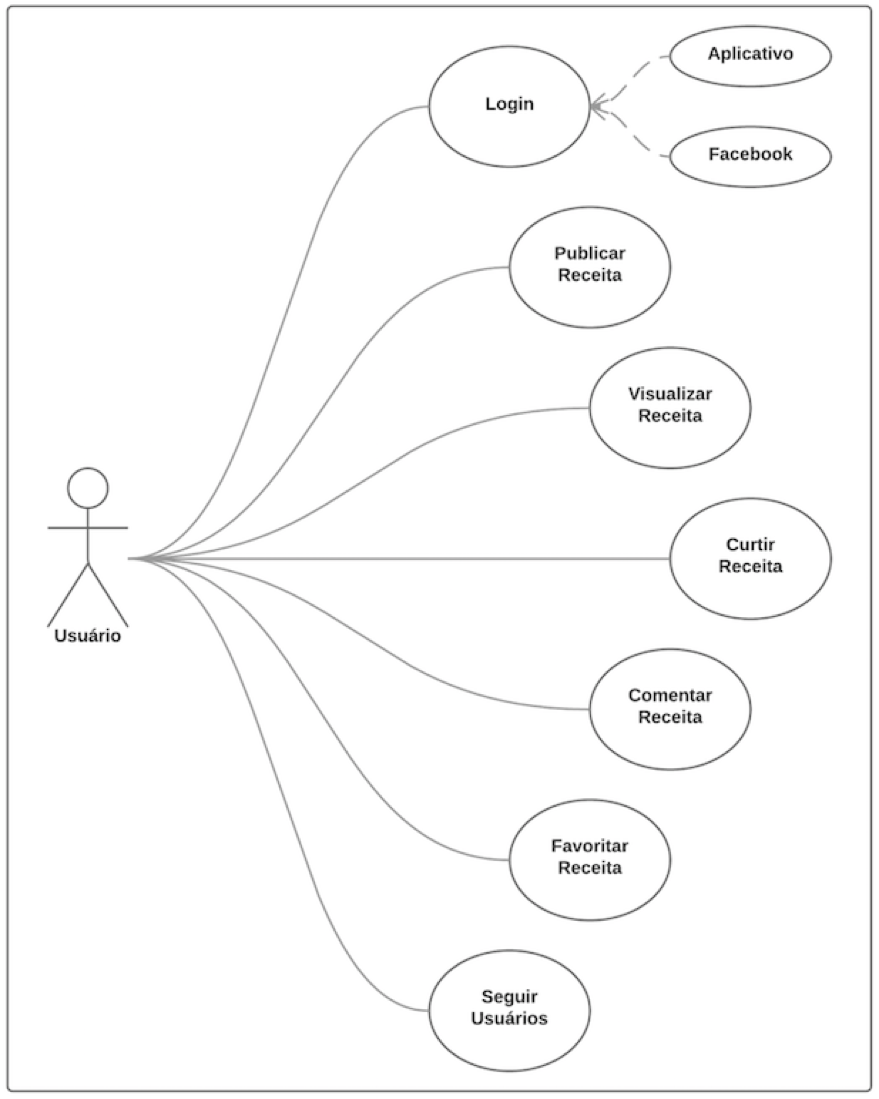
\includegraphics[scale=0.7]{imagens/figura8.png}
	\legend{Fonte: Elaborada pelo autor}
\end{figure}


\subsubsection{Descrição dos casos de uso} \label{sec:vegood: descricao-dos casos-de-uso}

A partir do diagrama mostrado na Figura \ref{fig:diagrama-de-caso-de-uso}, foram criados os seguintes casos de uso:

\begin{lista}
	\item \textbf{Caso de Uso 01 - LOGIN};
	\item \textbf{Caso de Uso 02 - PUBLICAR RECEITA};
	\item \textbf{Caso de Uso 03 - VISUALIZAR RECEITA};
	\item \textbf{Caso de Uso 04 - CURTIR RECEITA};
	\item \textbf{Caso de Uso 05 - COMENTAR RECEITA};
	\item \textbf{Caso de Uso 06 - FAVORITAR RECEITA};
	\item \textbf{Caso de Uso 07 - SEGUIR USUÁRIOS};
\end{lista}

Os documentos com as especificações completas estão disponíveis no apêndice \ref{apendice:a} deste trabalho.


\subsection{Diagrama de Classes}

O Diagrama de Classes descreve, em seu conteúdo, as classes e os seus relacionamentos. Em adendo, apresenta ainda o modelo de dados físico do aplicação, Figura \ref{fig:diagrama-de-classes}.

\begin{figure}[H]
	\caption{\label{fig:diagrama-de-classes}Diagrama de classes do Vegood}
	\centering
	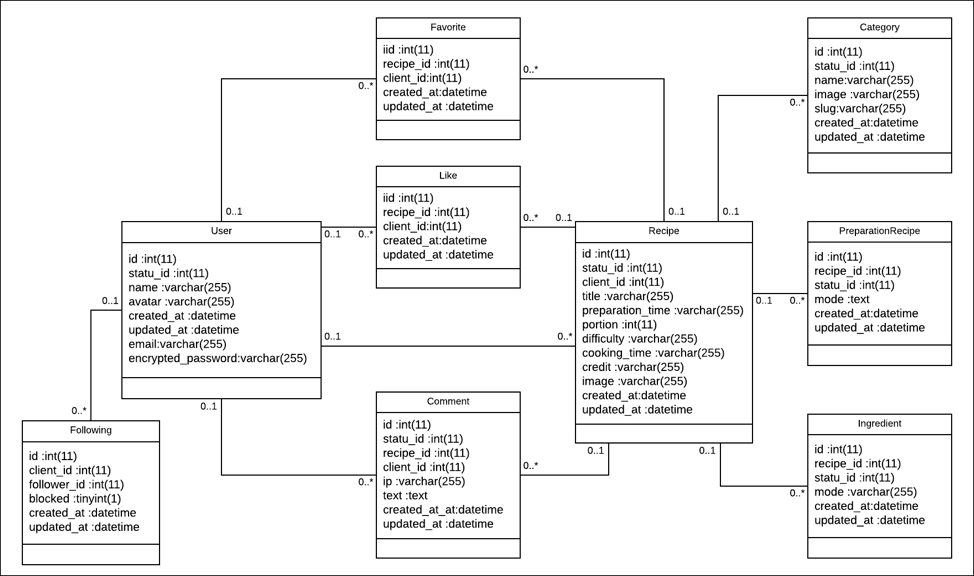
\includegraphics[scale=0.9]{imagens/figura9.png}
	\legend{Fonte: Elaborada pelo autor}
\end{figure}



\section{Desenvolvimento}
Nesta seção apresentamos uma visão dos passos e estrutura de projeto utilizando o framework híbrido Ionic. 


\subsection{Preparando o ambiente de trabalho} \label{sec:vegood:Funcionalidades}
Na implementação do código fonte foi utilizado o Sublime Text 3, um editor de texto projetado para ser simples, rápido, flexível e fácil de usar. Registramos que foram requeridas algumas dependências no desenvolvimento deste projeto. 

A seguir, serão descritas, de forma sequencial, as etapas necessárias a preparação do ambiente de trabalho.

Para obter o Ionic, precisamos do Node.JS, que é uma plataforma de desenvolvimento de aplicações utilizando Javascript, instalado na máquina, pois o processo é feito via NPM, um gerador de pacotes do Node.Js . Após instalar o Node.JS com sucesso, é indicado que se adicione os SDKs (\textit{Software Development Kit}) da(s) plataforma(s) com que se deseja trabalhar (Android, IOS, Windows Phone). Cada plataforma possui um processo de instalação diferenciado, lembrando que para utilizar e compilar versões para iOS é necessário que se utilize um notebook da linha Mac, do fabricante Apple. Com o Node.Js instalado, o utilitário terminal deve ser utilizado para a instalação do Ionic, através do comando ”npm install  -g ionic”. Ao final desta execução o ambiente Ionic torna-se disponível e acessível por meio do comando externo “ionic”. Para uma confirmação, a execução do comando “ionic --version“, exibe a versão instalada.

Usando o gerador do Ionic CLI para a criação de um novo projeto, informamos o template desejado e um modelo é gerado com os componentes iniciais do template escolhido. Para tal é utilizado o seguinte comando: “ionic start nomedoapp [template]“, onde tabs é o parâmetro padrão para template , que pode ser substituído pelos parâmetros sidemenu ou blank.

Para testar o aplicativo, o Ionic  CLI disponibiliza o comando “ionic serve [opção]“ que inicia um servidor de desenvolvimento local que pode ser visualizado em seu navegador padrão.. Esse comando também inicia o Live Reload, recurso que é utilizado para monitorar as mudanças feitas na aplicação. Com ele, qualquer alteração no arquivo do projeto irá atualizar automaticamente o browser. Uma opção adicional para a  visualização do projeto é o comando “ionic serve --lab“, que simula as telas em Android e IOS, lado a lado.

Após as etapas descritas acima, o ambiente se encontra pronto para o inicio do desenvolvimento.

\subsubsection{Estrutura do sistema}
Em um projeto utilizando Ionic Framework é gerada uma estrutura de diretórios, comum a todos os projetos (Figura 10).

\begin{figure}[H]
	\caption{\label{fig:estrutura-de-diretorios-do-projeto}Estrutura de diretórios do projeto Vegood}
	\centering
	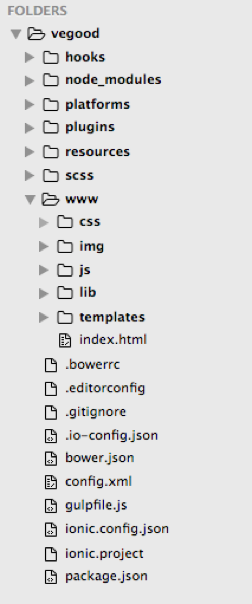
\includegraphics[scale=1]{imagens/figura10.png}
	\legend{Fonte: Elaborado pelo autor}
\end{figure}


\subsection{Interface do aplicativo}
Descrevemos as principais telas da interface gráfica da aplicação Vegood.

\subsubsection{Tela de login}
Logo que a aplicação é aberta, a tela de login é apresentada e o usuário tem 3 possibilidades de ação: 
\begin{lista}
	\item Fazer o login pelo próprio aplicativo (usando os dados necessários, se já possuir uma conta);
	\item fazer login usando o facebook (onde o aplicativo pede autorização para usar as credenciais do facebook para prosseguir o acesso ao aplicativo);
	\item  Criar uma nova conta;
\end{lista}

\begin{figure}[H]
	\caption{\label{fig:tela-de-login}Tela de login}
	\centering
	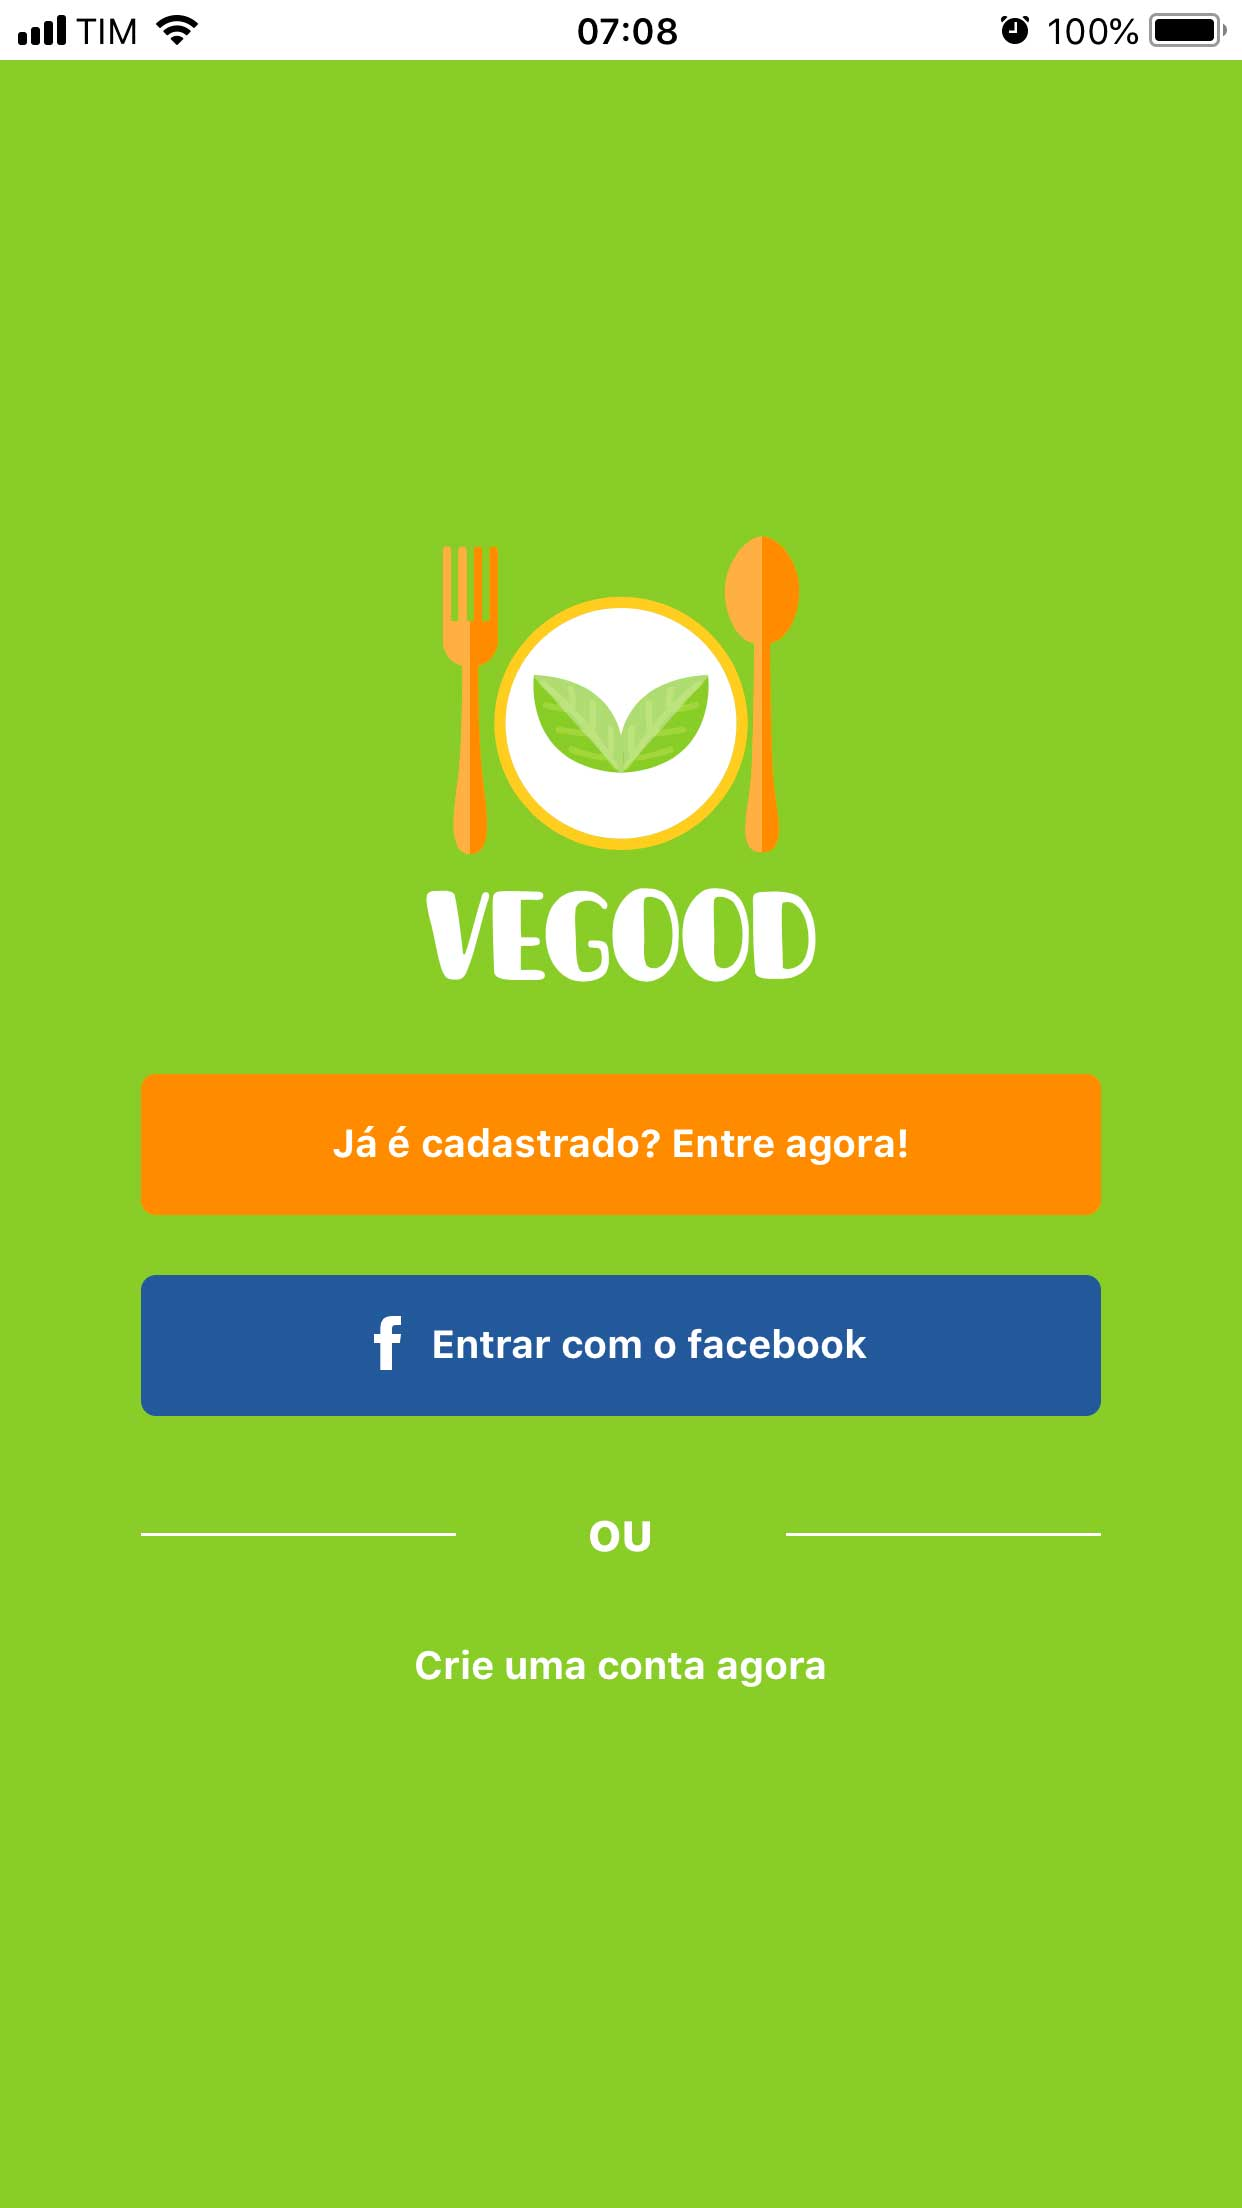
\includegraphics[scale=0.15]{imagens/figura11.jpg}
\end{figure}




\subsubsection{Tela de cadastro}
Essa tela por meio da qual o usuário cria sua conta para ter acesso e usufruir de todas funcionalidades do aplicativo. Com exceção de cadastrar a foto de perfil, todos os campos são obrigatórios e devem ser preenchidos para a conclusão do cadastro.

\begin{figure}[H]
	\caption{\label{fig:tela-de-1}Tela de cadastro}
	\centering
	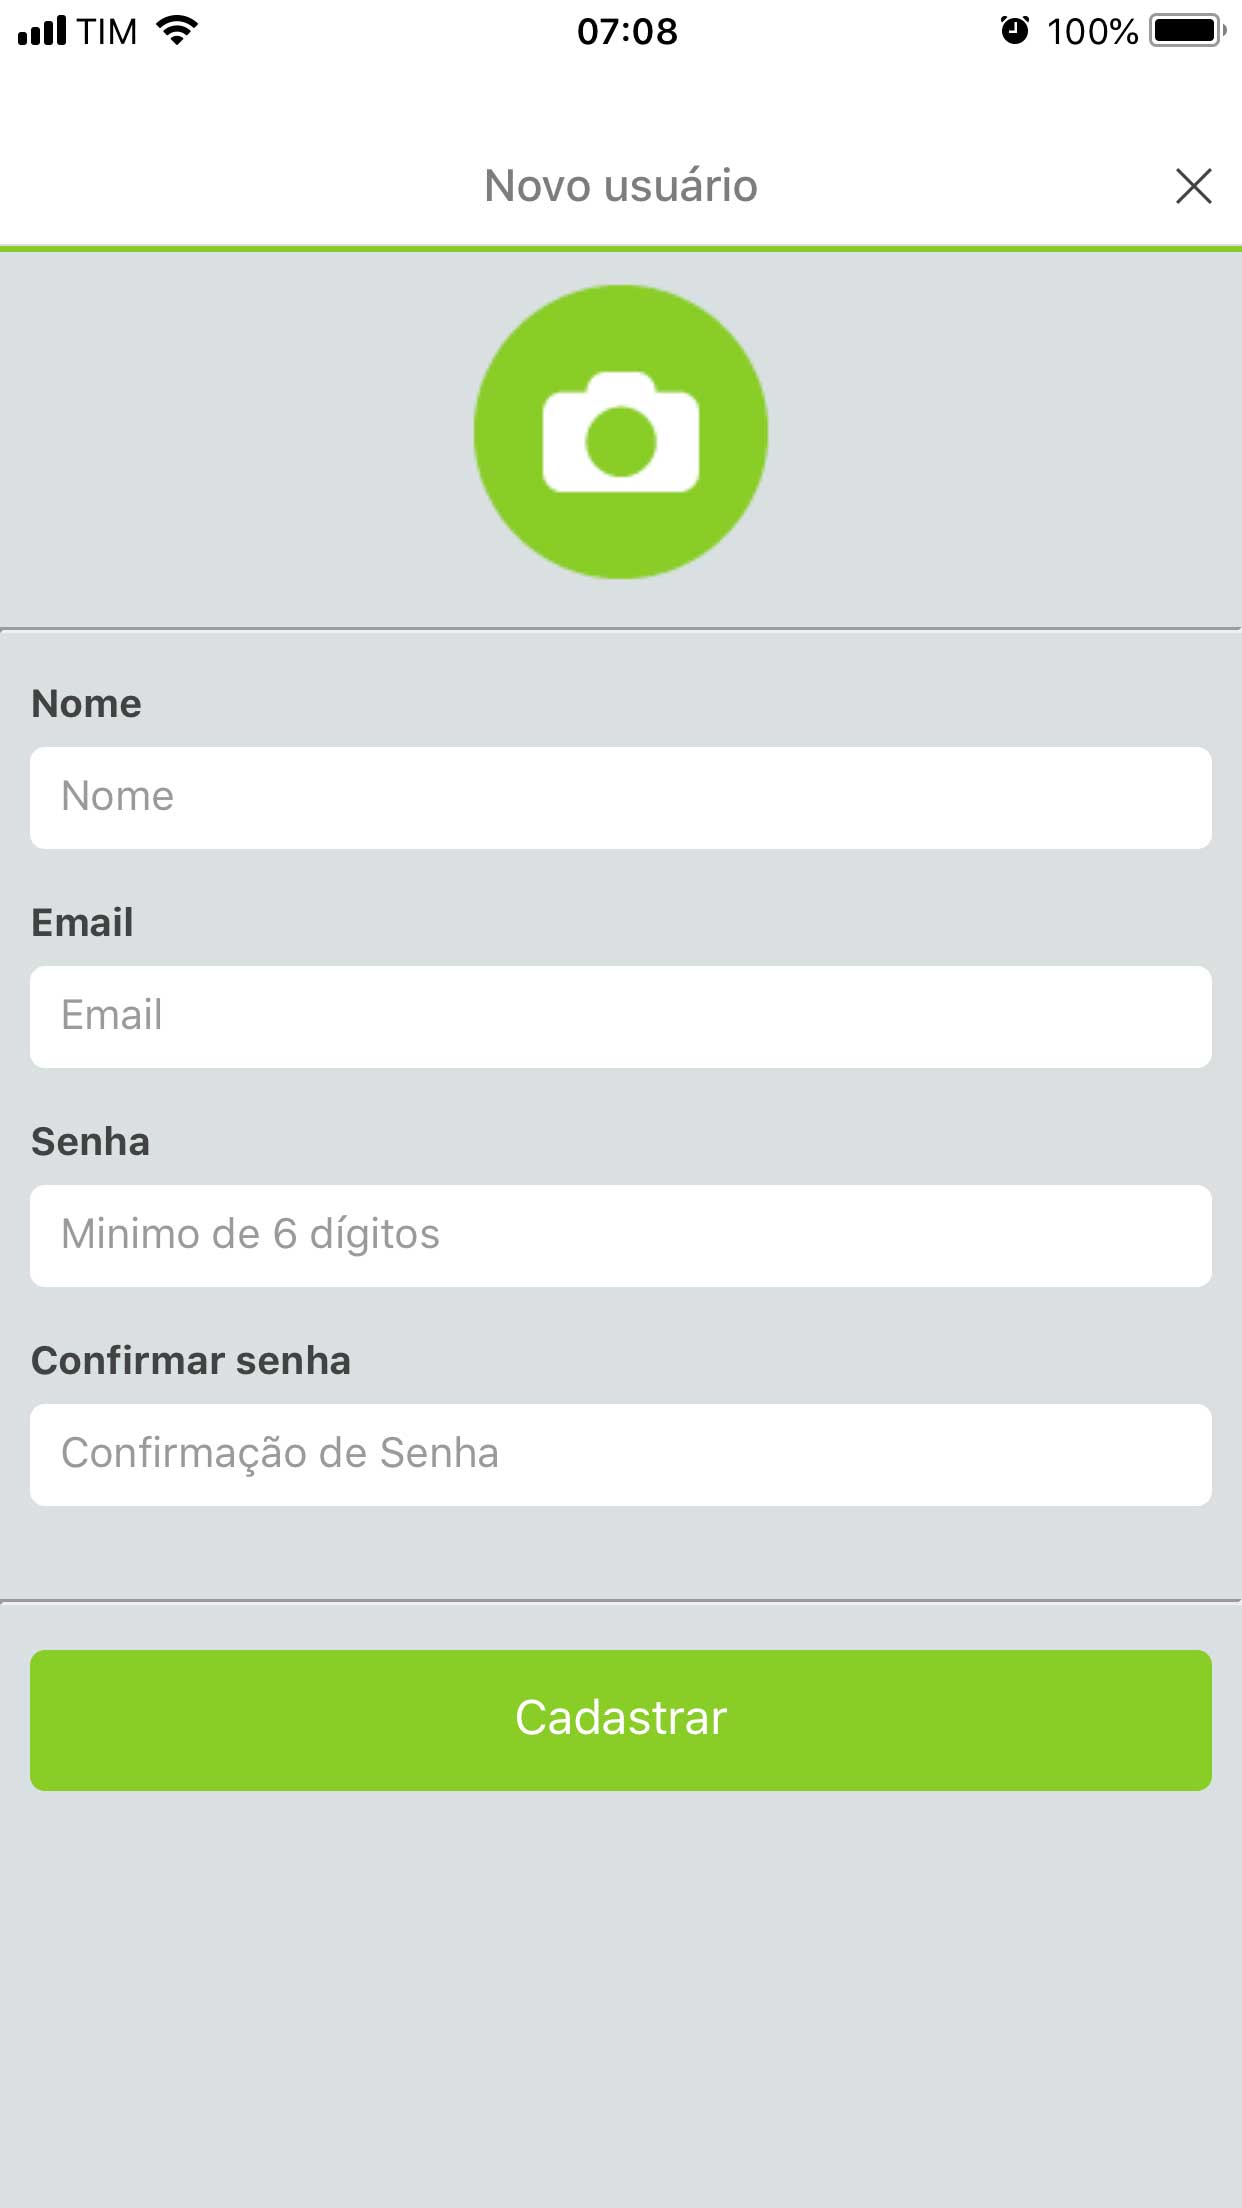
\includegraphics[scale=0.15]{imagens/figura12.jpg}
\end{figure}



\subsubsection{Tela principal}
Após a autenticação do usuário, a aplicação apresenta a tela principal com um \textit{feed} de receitas publicadas, onde o usuário pode interagir com as mesmas, clicando no nome do usuário que publicou a receita e se encaminhando ao seu perfil. Com apenas  um clique, o usuário também pode curtir, comentar e até mesmo favoritar as receitas. Além disso, para obter mais informações de uma determinada receita, basta clicar em uma delas e uma nova tela surge, com todas as informações.

Nessa mesma tela, também podemos ver um menu em tabs na parte inferior do aplicativo, que representam as opções de exibições: Inicio, Categorias, Enviar receita, Conta e Mais.

\begin{figure}[H]
	\caption{\label{fig:tela-de-2}Tela principal}
	\centering
	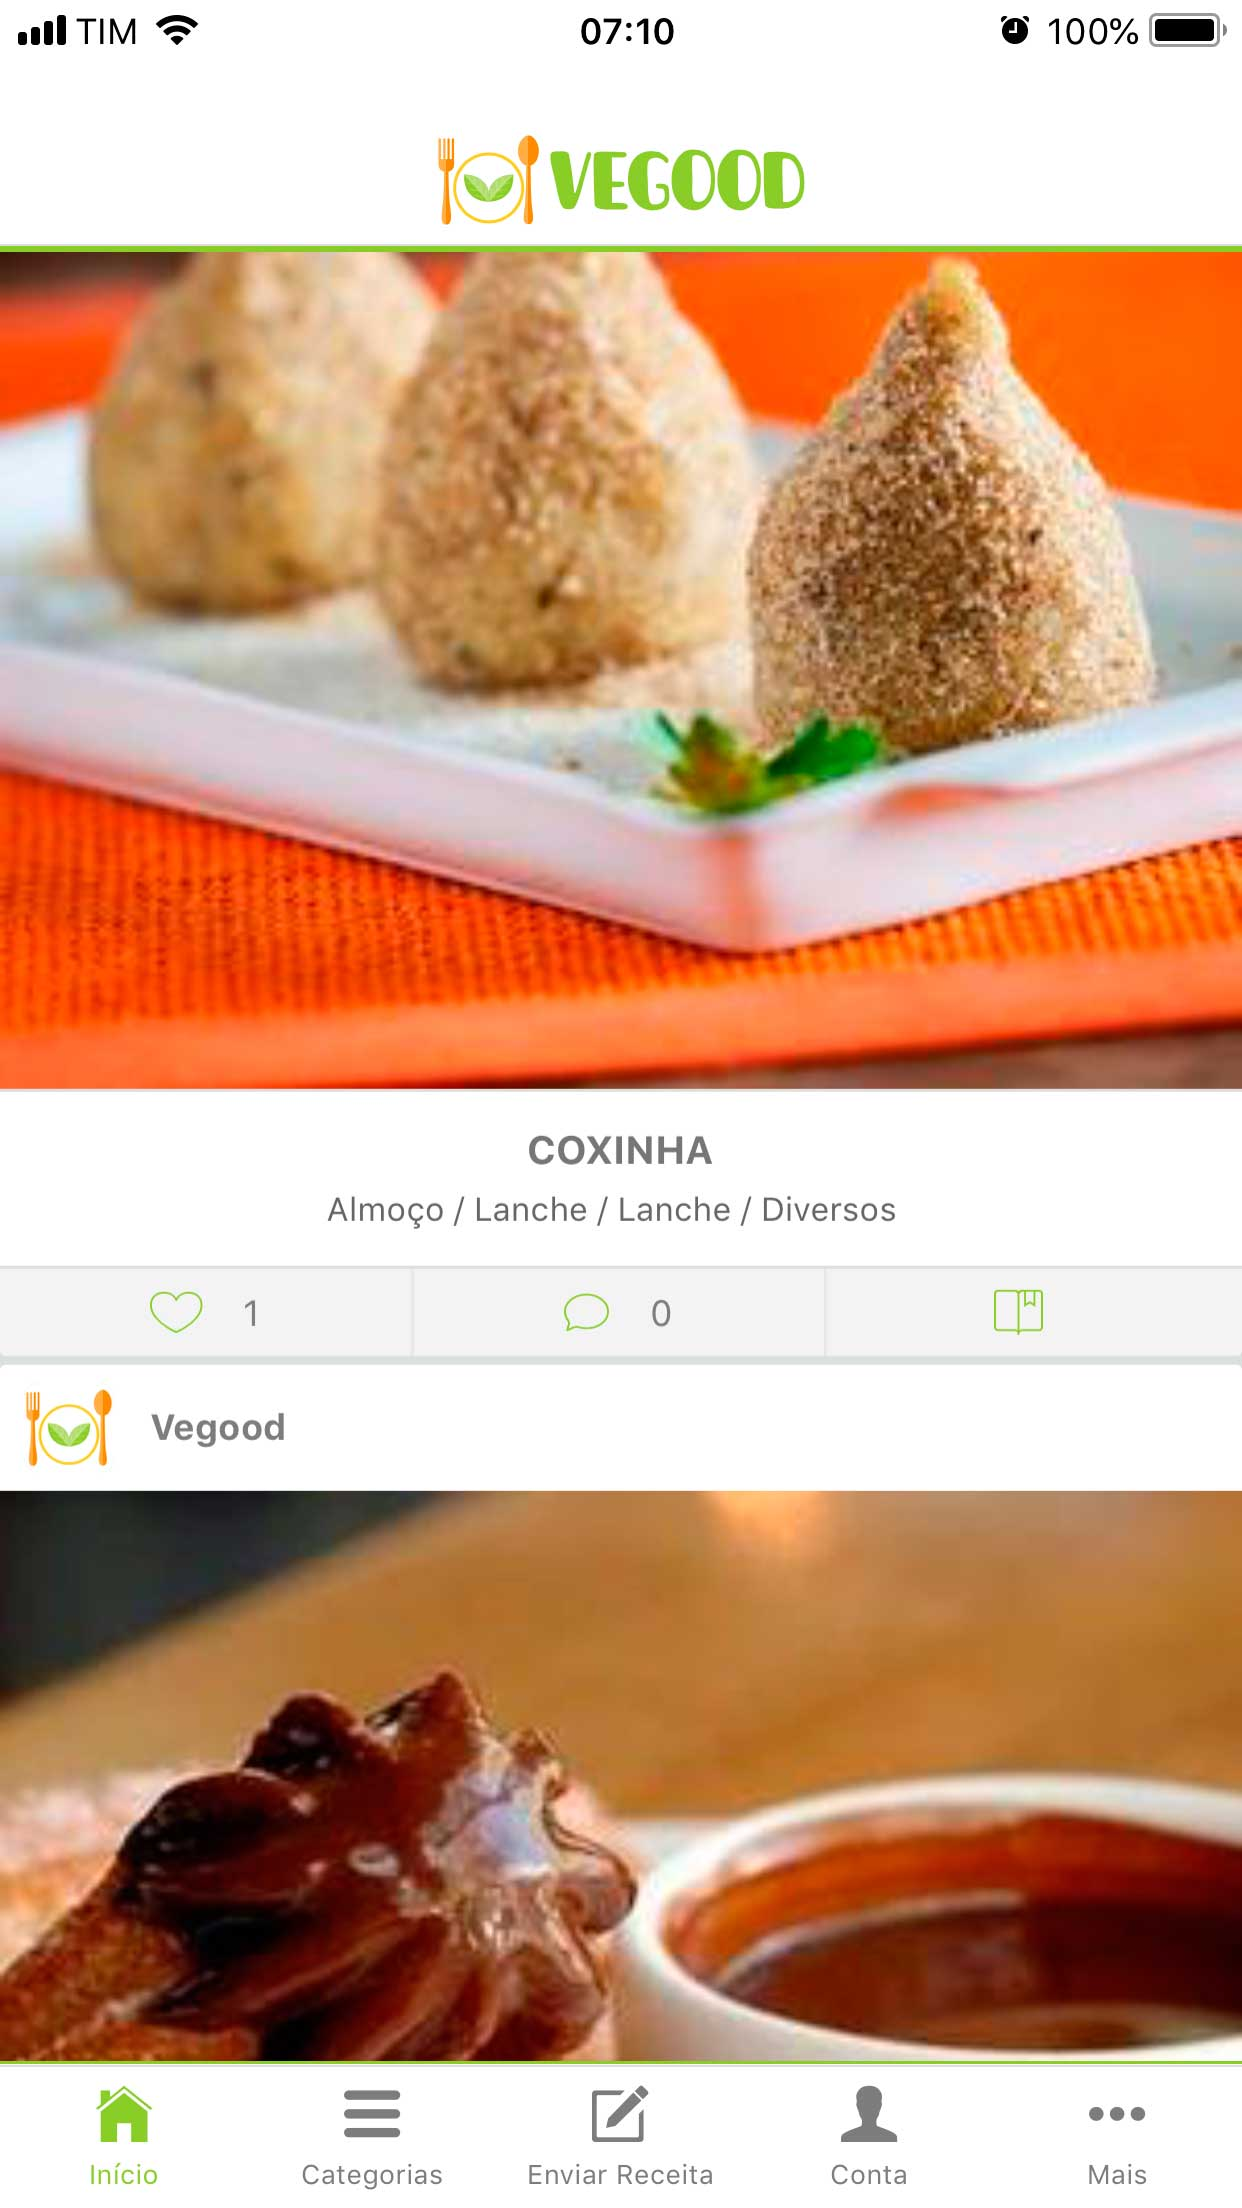
\includegraphics[scale=0.15]{imagens/figura13.jpg}
\end{figure}

\subsubsection{Tela interna de uma receita}
Nessa tela, o usuário pode fazer praticamente as mesmas coisas da tela principal, podendo clicar no nome do usuário que publicou a receita e ir para o seu perfil. Com um clique, o usuário também pode curtir, comentar e até mesmo favoritar as receitas. A parte mais importante dessa tela são as informações sobre a receita, onde o usuário pode ver, por exemplo, o tempo de preparo e cozimento, o rendimento e a dificuldade, além de ter todas as informações de ingredientes necessários e modo de preparo para fazer a receita.

\begin{figure}[H]
	\caption{\label{fig:tela-de-3}Tela interna de uma receita}
	\centering
	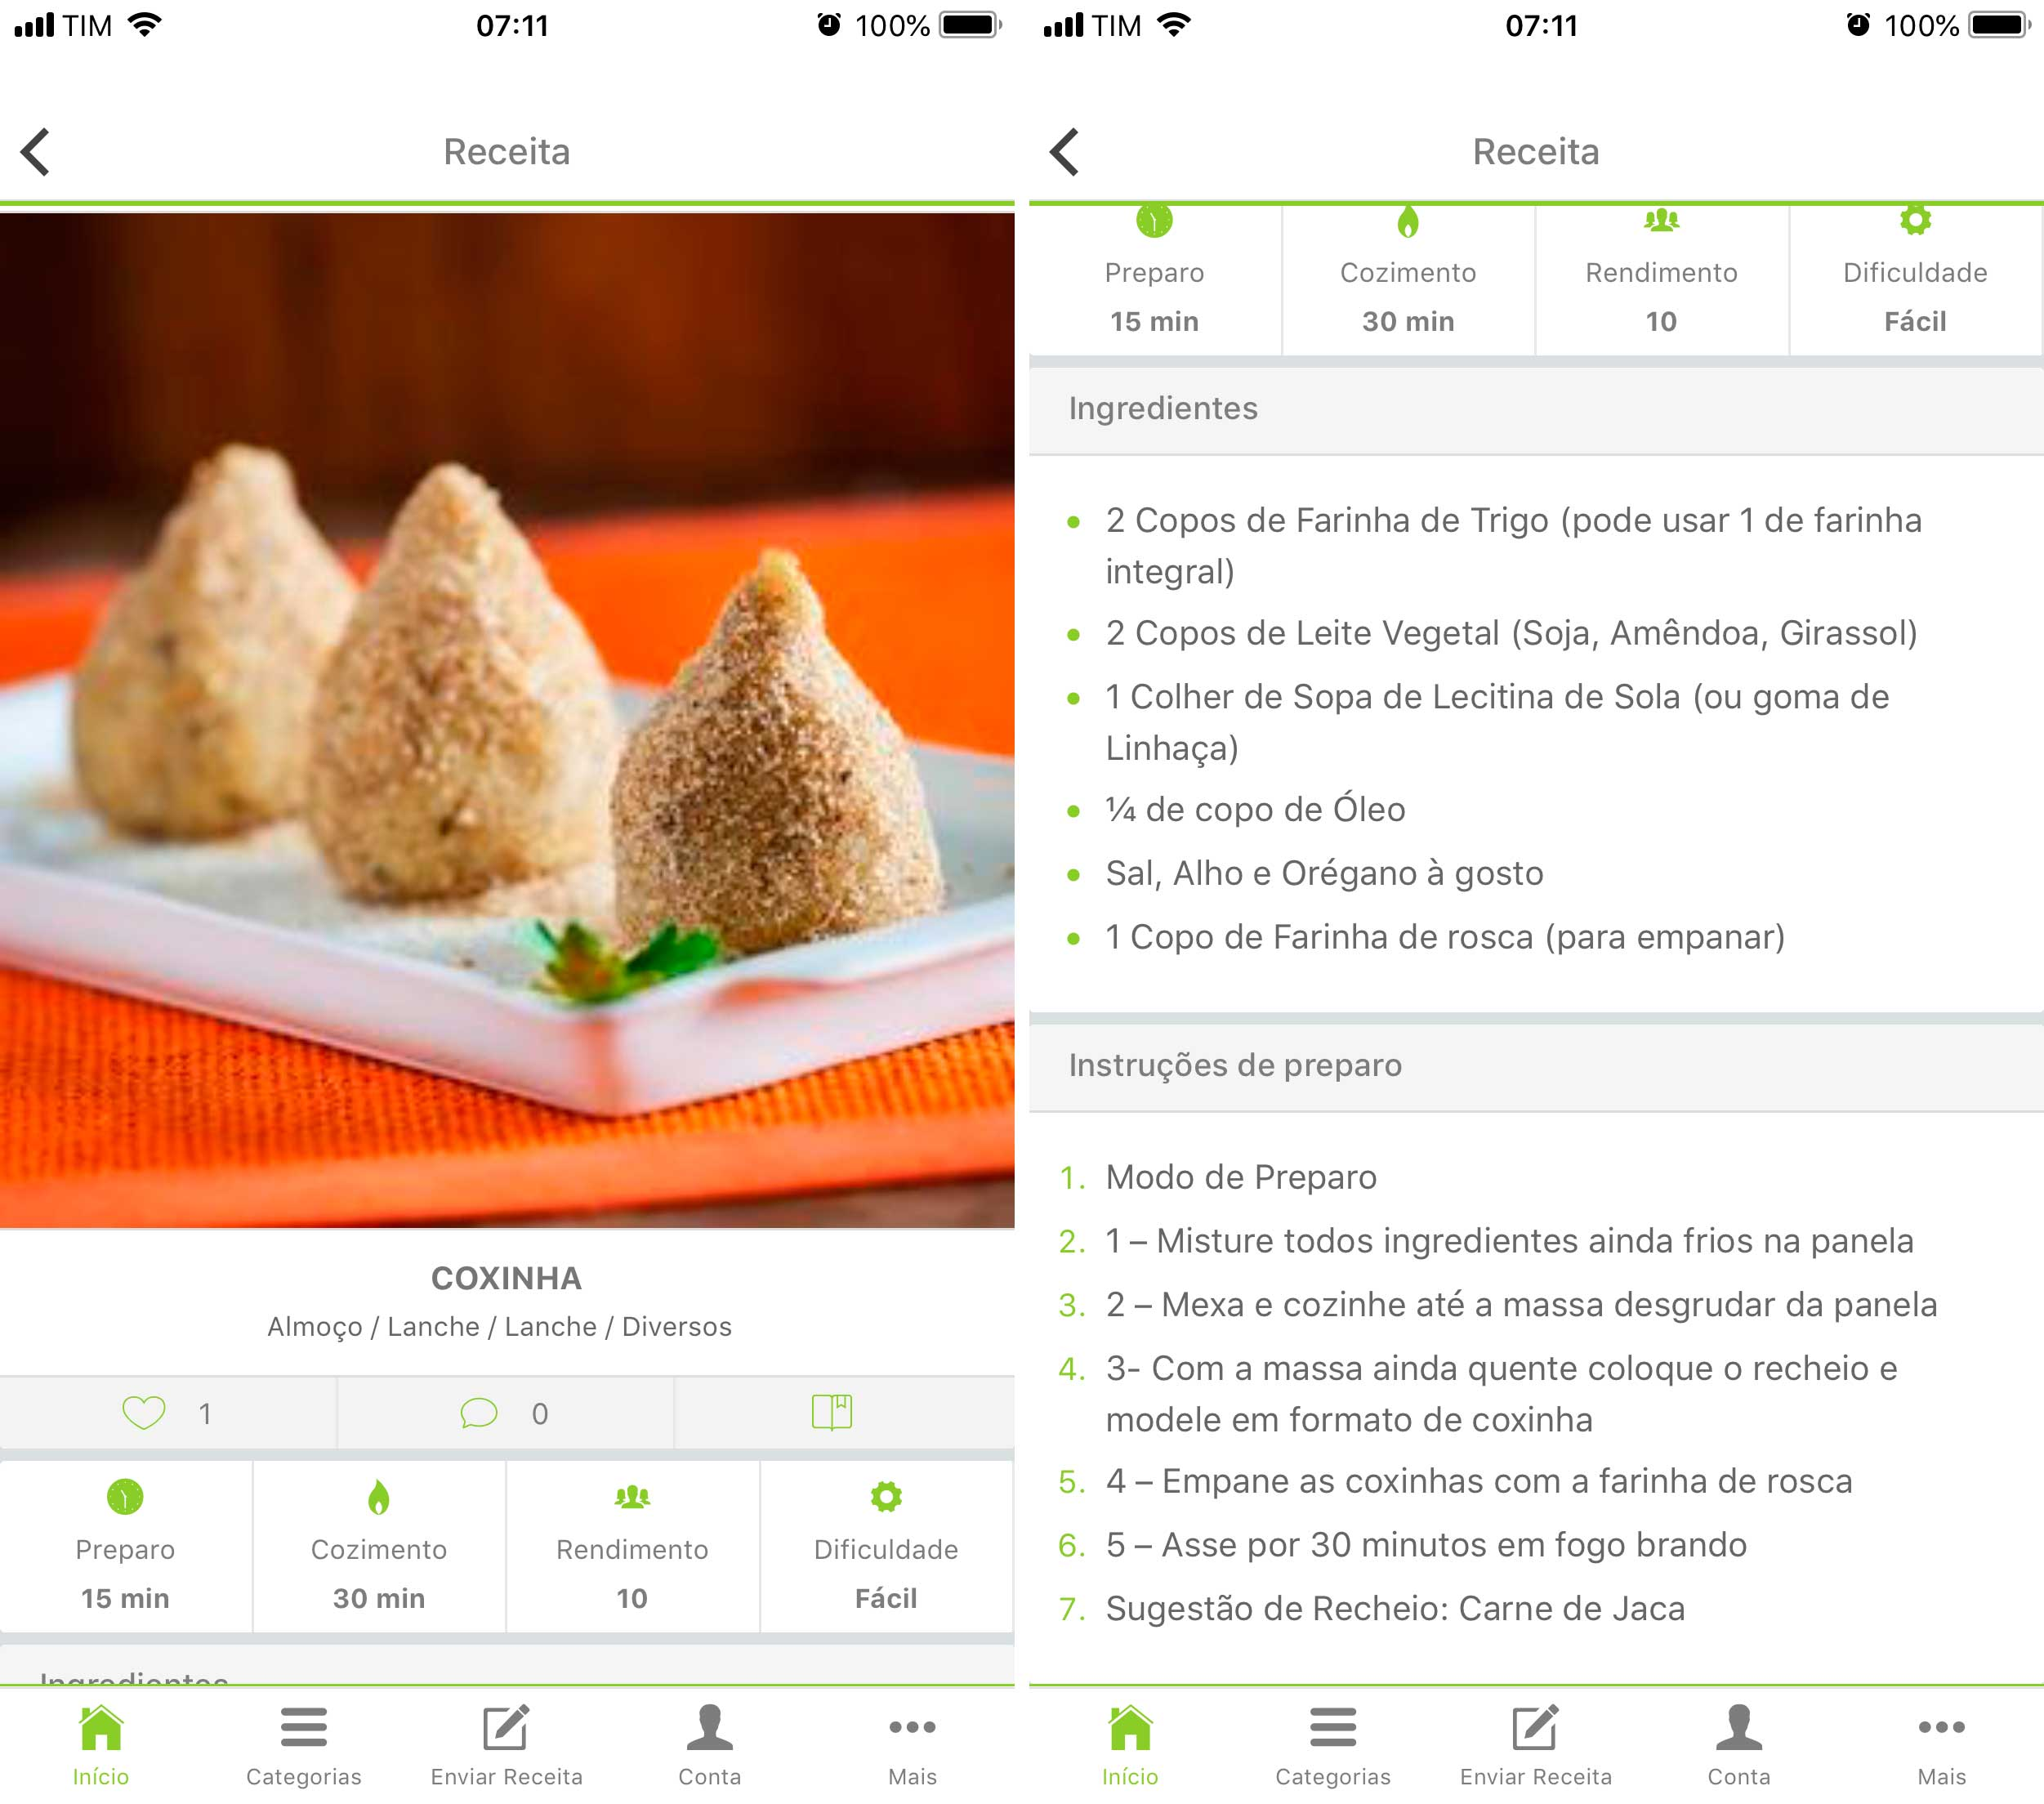
\includegraphics[scale=0.15]{imagens/figura14.jpg}
\end{figure}

\subsubsection{Tela de categorias}
Na tela de categorias o usuário tem disponível 5 categorias: almoço, café da manhã, jantar, lanche e outros. Com as categorias divididas dessa forma, fica facilitada a localização de alguma receita, de acordo com o tipo de refeição que se deseja  aprender.

Ao se clicar em uma categoria uma nova tela é apresentada, contendo todas as receitas relacionadas à categoria selecionada e, na parte superior, a quantidade de receitas que aquela categoria possui

\begin{figure}[H]
	\caption{\label{fig:tela-de-4}Tela de categorias}
	\centering
	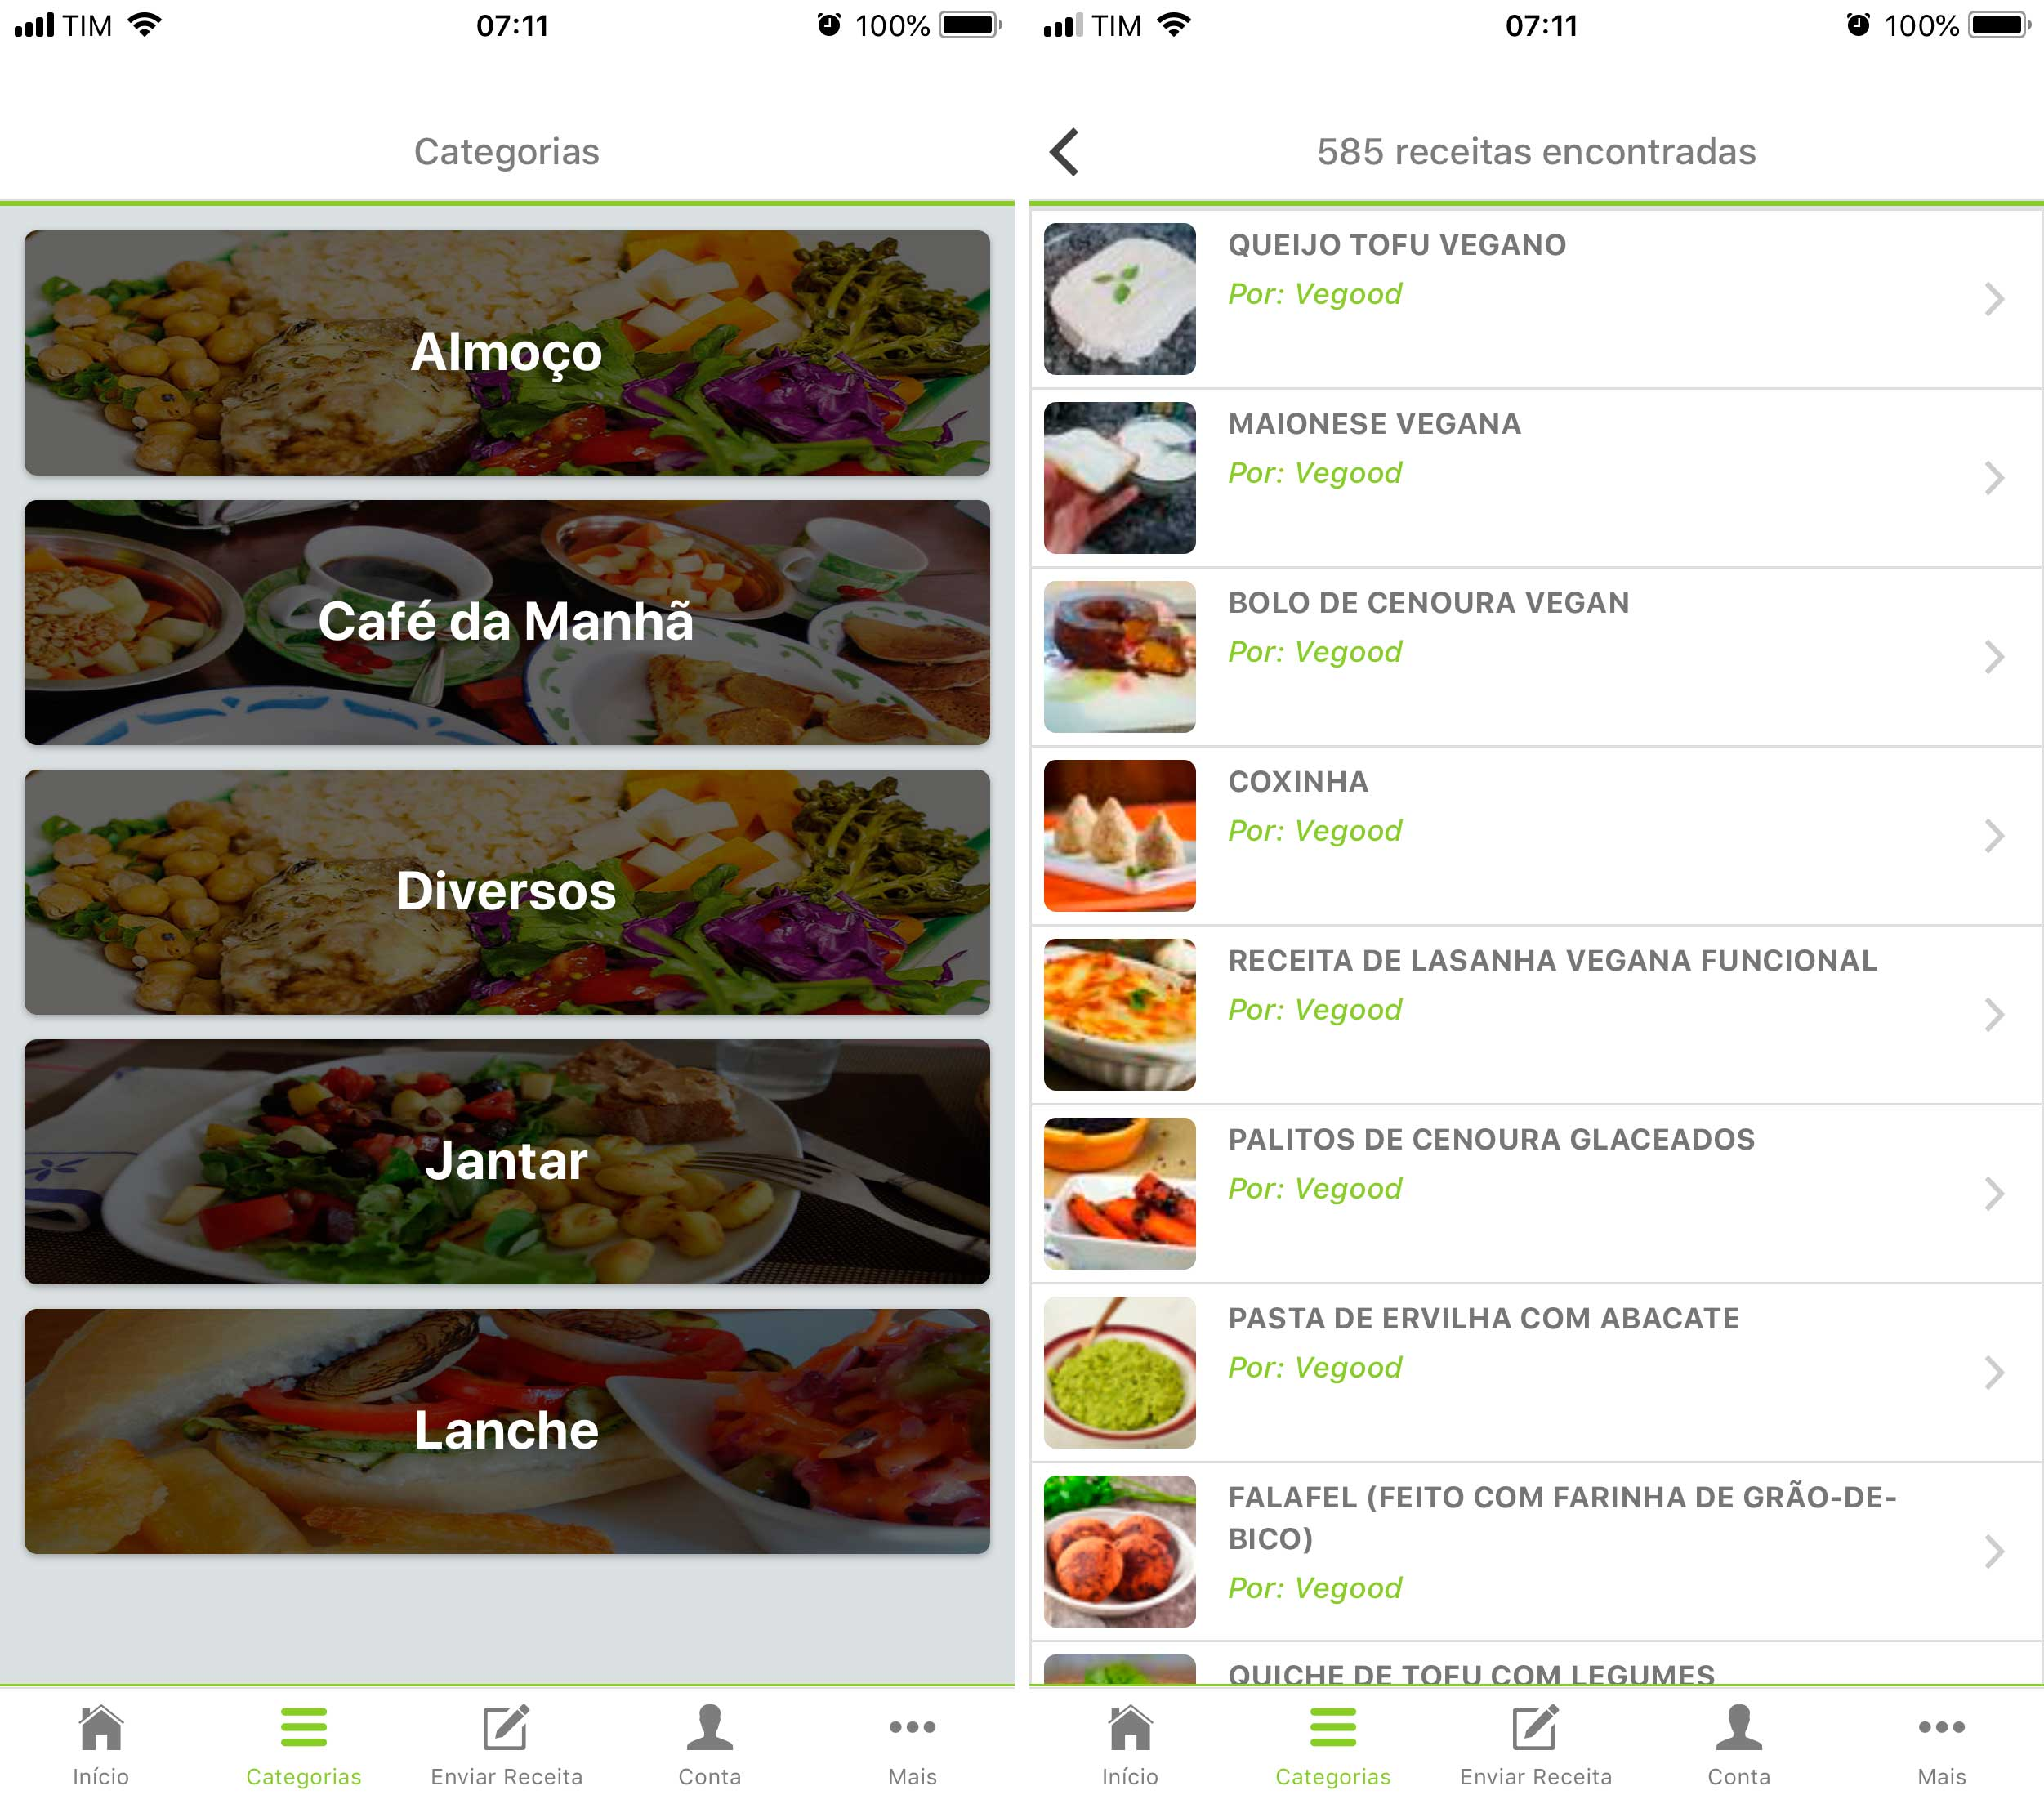
\includegraphics[scale=0.15]{imagens/figura15.jpg}
\end{figure}

\subsubsection{Tela de enviar uma receita}
Na tela de enviar receita, o usuário tem disponível um formulário bem simples e objetivo com os campos necessários para publicar uma receita. Nesse formulário  há a possibilidade de se usar a câmera do próprio celular para capturar uma foto ou selecionar dos seus arquivos uma imagem para a receita. O usuário, além da foto, pode cadastrar de forma prática e direta o nome da receita, como também selecionar uma ou mais categorias, tempo de preparo, tempo de cozimento, rendimento, dificuldade de execução, os ingredientes e o modo de preparo.

\begin{figure}[H]
	\caption{\label{fig:tela-de-5}Tela de enviar uma receita}
	\centering
	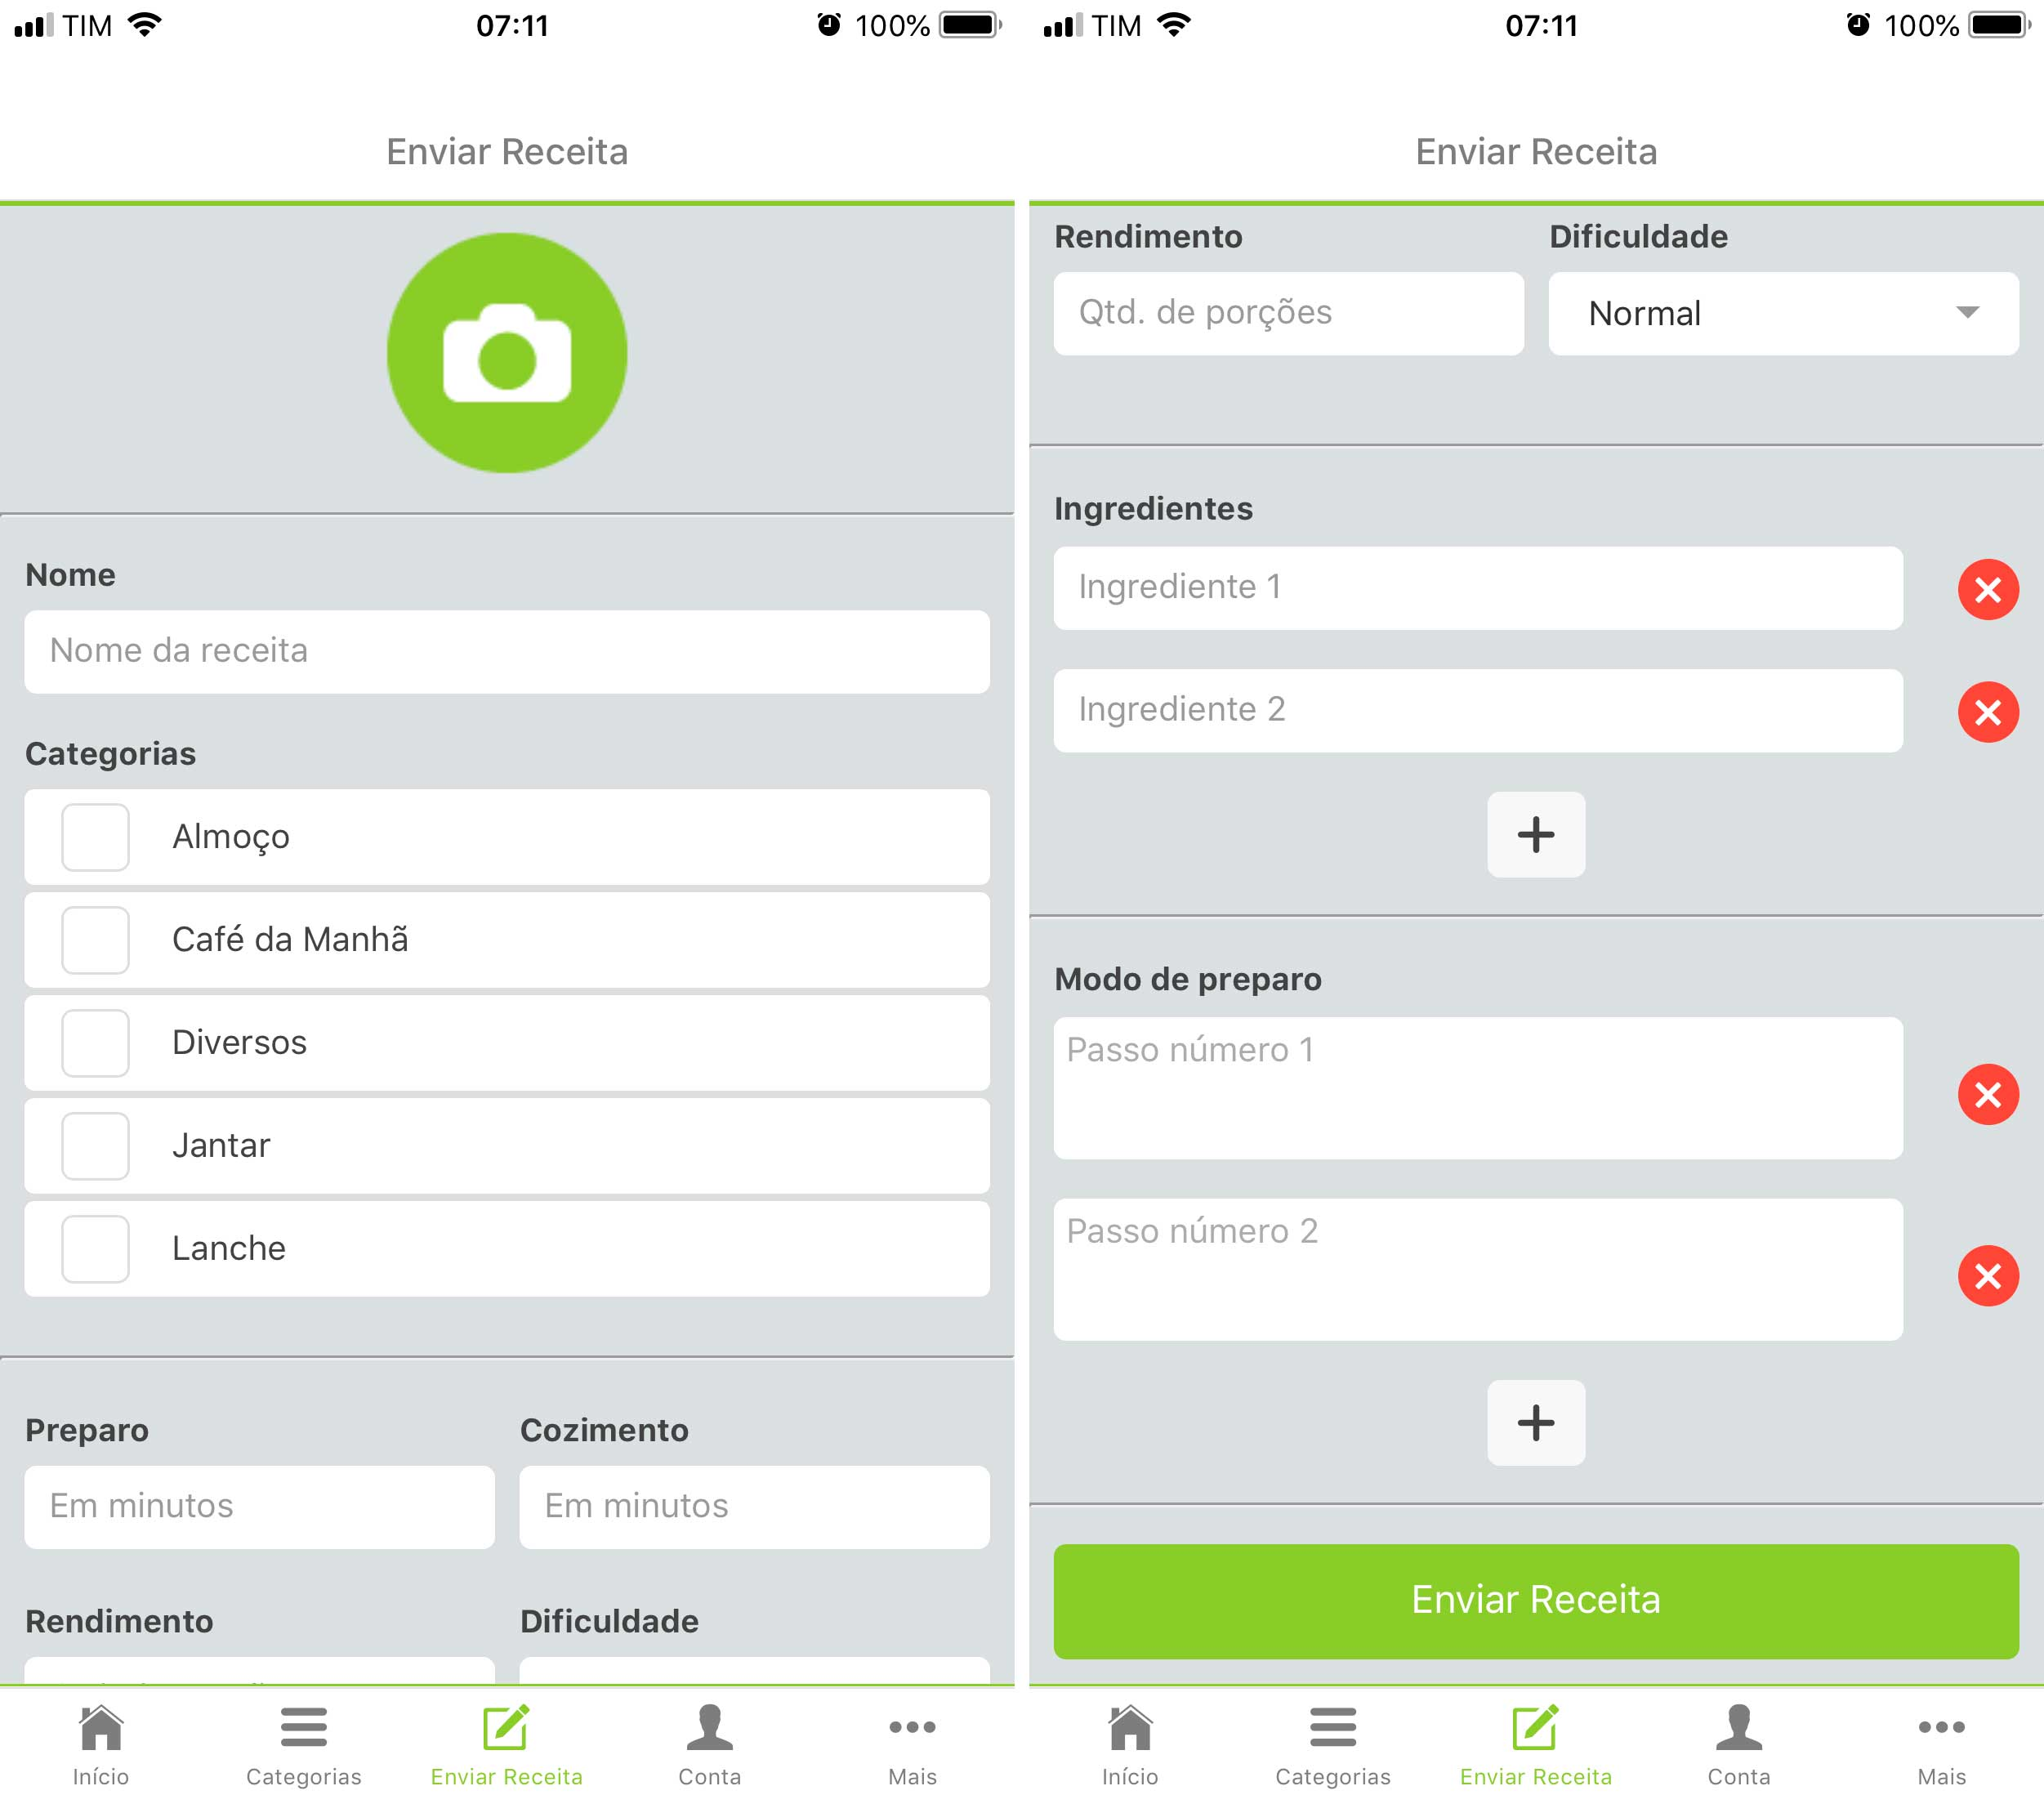
\includegraphics[scale=0.15]{imagens/figura16.jpg}
\end{figure}

\subsubsection{Tela de perfil}
A tela de perfil é bem simples. O usuário pode ver as receitas que favoritou bem como editar o seu próprio perfil. É possível ainda ver a quantidade a lista das receitas que publicou,os seus seguidores e a quem está seguindo.

No topo da tela existe uma opção para edição dos seus dados pessoais.

\begin{figure}[H]
	\caption{\label{fig:tela-de-6}Tela de perfil}
	\centering
	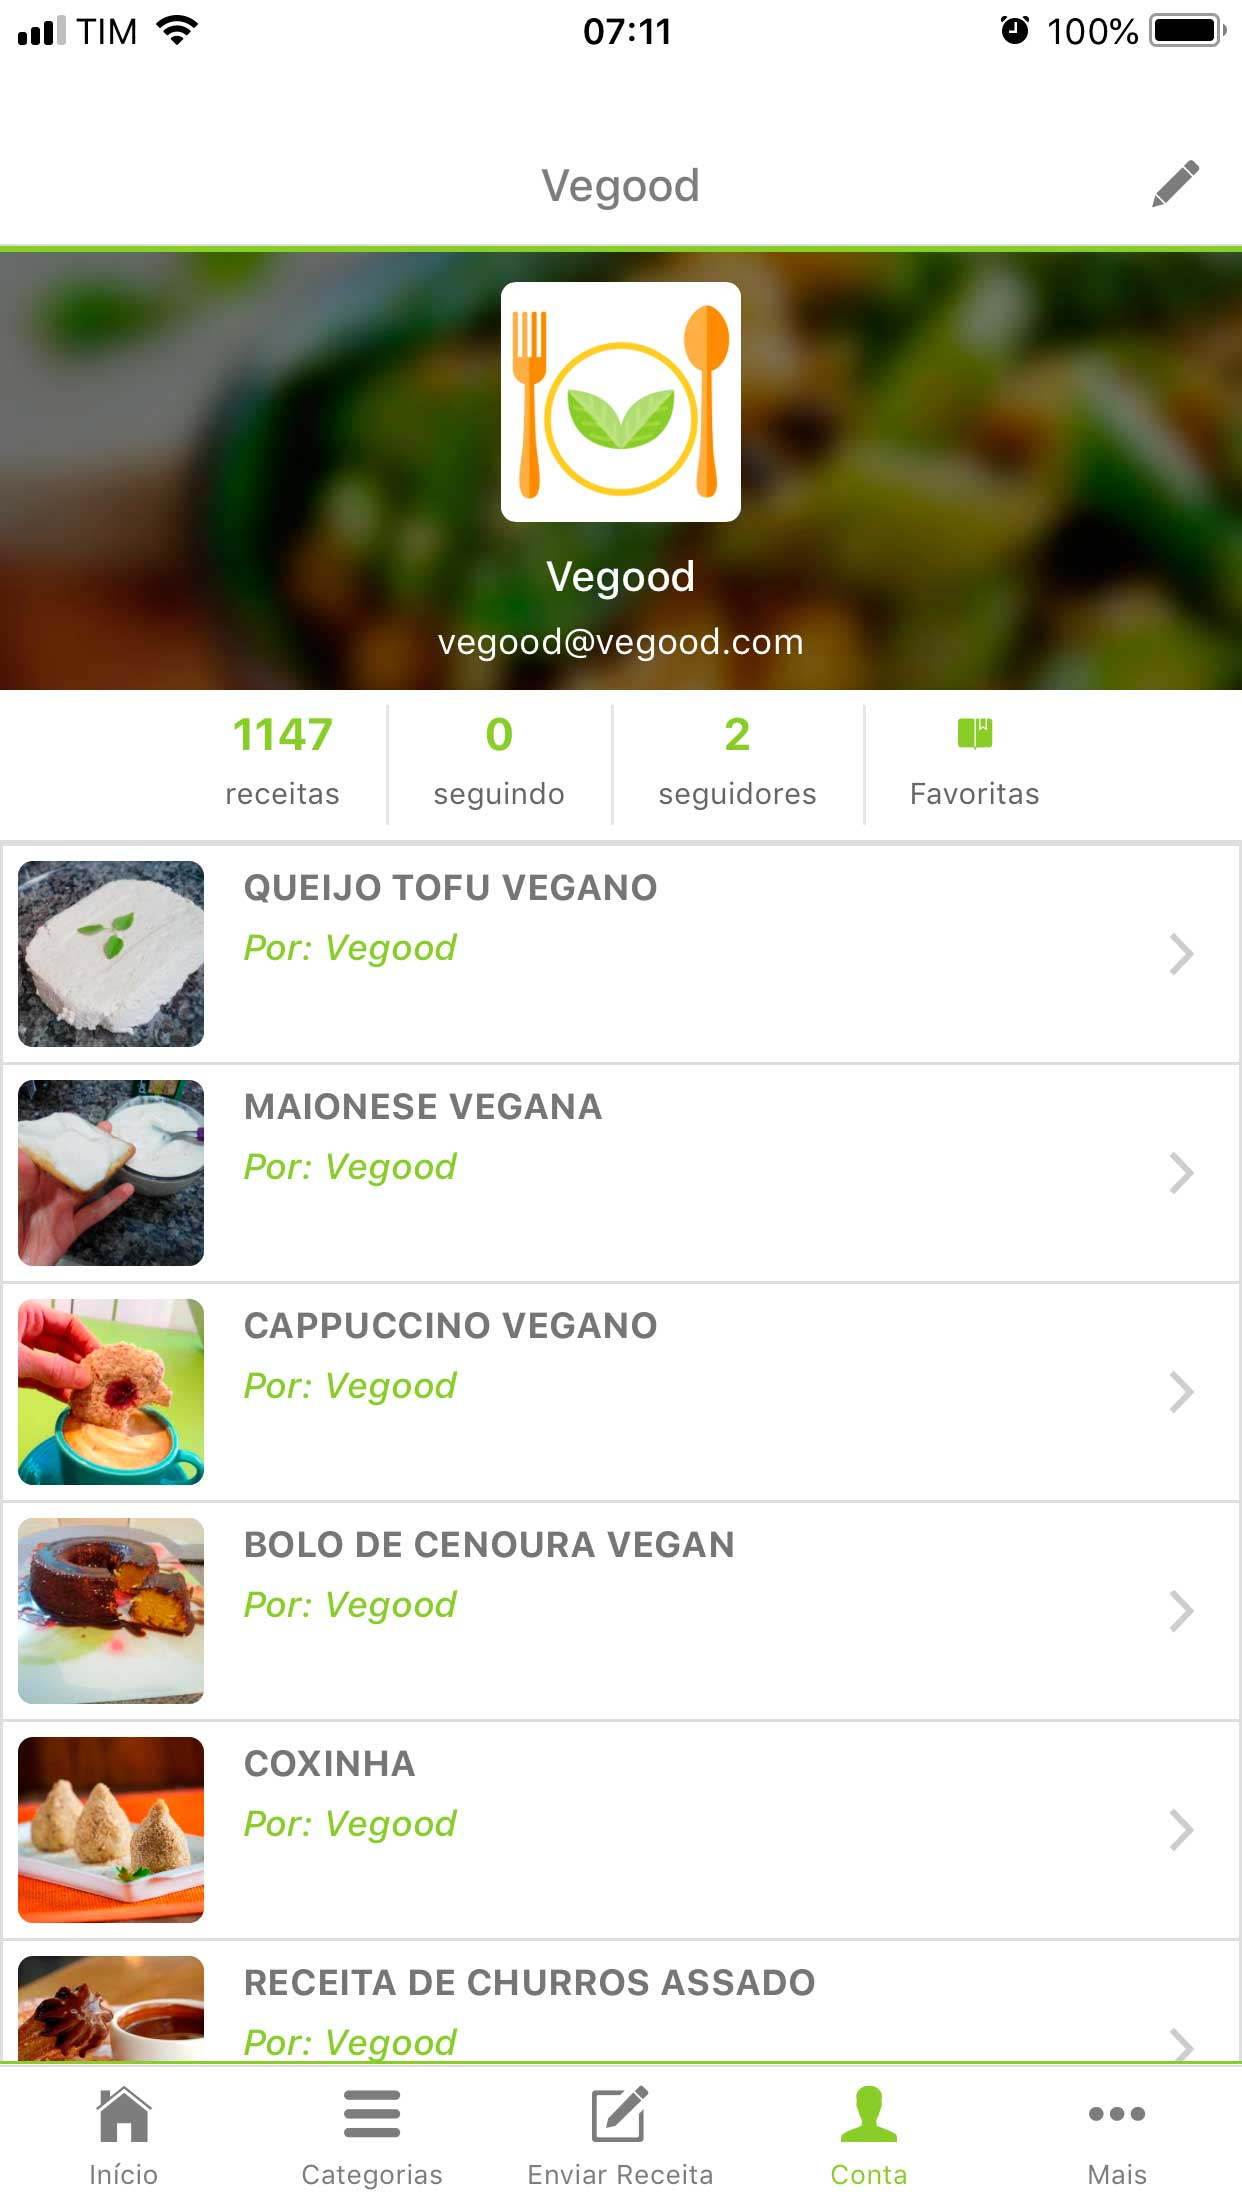
\includegraphics[scale=0.15]{imagens/figura17.jpg}
\end{figure}

% ----------------------------------------------------------
% Conclusão
% ----------------------------------------------------------

\chapter{Conclusão}

% O desenvolvimento do presente trabalho foi de grande importância para aumentar os conhecimentos do tema proposto. Analisando aspectos relacionados as redes sociais e dispositivos móveis, usando especialmente essas abordagens no contexto do veganismo e vegetarianismo. Desse modo, entender a relação dessas variáveis foi muito útil para a compreensão e desenvolvimento do aplicativo no decorrer do trabalho.

% O trabalho teve como objetivo geral o desenvolvimento de um aplicativo de rede social, com o proposito de compartilhar conhecimentos e informações de receitas culinárias, principalmente pelo publico vegetariano e vegano. 


O trabalho teve como objetivo geral o desenvolvimento de um aplicativo de rede social para compartilhamento de conhecimentos e informações de receitas culinárias, principalmente pelo publico vegetariano e vegano, que demonstrou ser de grande importância para aumentar os conhecimentos acerca do tema proposto. Analisando aspectos relacionados as redes sociais e dispositivos móveis, usando especialmente essas abordagens no contexto do veganismo e vegetarianismo. Desse modo, entender a relação dessas variáveis foi muito útil para a compreensão e desenvolvimento do aplicativo no decorrer do trabalho.

Foi feita uma imersão no contexto abordado, possibilitando o desenvolvimento do aplicativo mobile, onde foi posto em balança se o mesmo seria desenvolvido de forma nativa ou hibrida usando a tecnologia do framework Ionic. Pensando de uma forma ágil para o que estava sendo proposto, conclui-se que era mais viável, inclusive pelo custo e tempo de desenvolvimento, que a utilização da tecnologia hibrida seria a solução mais adequada, onde supriria todas as necessidades durante o desenvolvimento e abrangeria as plataformas mobiles mais utilizadas.

Ao final do desenvolvimento, aplicativo passou por testes e atendeu bem as expectativas, gerando resultados satisfatórios, concluindo que o problema relatado sobre as dificuldade de encontrar variedades de receitas em um só local foi solucionada com a criação do aplicativo, permitindo assim, que os objetivos propostos fossem realmente alcançados.

Para finalizar, a partir do que foi desenvolvido para este trabalho,  é possível realizar pesquisas mais elaboradas para ter uma visão mais detalhada, criando estrategias para crescimento do aplicativo. 

% Como o aplicativo desenvolvido trata-se de um MVP (\textit{Minimum Viable Product}), dentre futuros aprimoramentos, os usuários poderão tirar duvidas por mensagens com nutricionistas e educadores físicos que possam vir a ser parceiros do aplicativo, inserção de vídeos e slides de fotos ao adicionar uma receita, compartilhar as receitas em outras redes sociais, notificações push.

% ----------------------------------------------------------
% Trabalhos Futuros
% ----------------------------------------------------------

%% Para tornar os trabalhos futuros um capítulo a parte, use \chapter{Trabalhos Futuros}
\chapter{Trabalhos Futuros}

% Para trabalho futuro, uma proposta seria o desenvolvimento de aplicativos nativos para dispositivos móveis.

A aplicação desenvolvida neste trabalho trata-se de um MVP (\textit{Minimum Viable Product}). Dentre outros futuros aprimoramentos, lista-se : 

\begin{lista}
   
     \item \textbf{Estudo de mercado}:  para ter uma visão mais detalhada do nicho desejado e criar estratégias de ação para o produto;
      \item \textbf{Versões nativas}: desenvolvimento de versões nativas mais aprimoradas do aplicativo;
% 	\item \textbf{Publicação do Aplicativo}: registro junto às maiores lojas de aplicativos mobiles, Google Play e Apple Store, para que a aplicação possa ser publicada;
	\item \textbf{Envio de notificações Push}: funcionalidade necessária para que a interação entre a aplicação e o usuário possa crescer;
	\item \textbf{Vídeos e slide de fotos}: possibilitar inserir vídeos ou mais de uma foto na criação de uma receita;
	\item \textbf{Compartilhamento das receitas}: funcionalidade que irá permitir que os usuários compartilhem suas receitas publicadas no aplicativo na sua página do Facebook, aumentando a visibilidade da aplicação para os amigos que ainda não possuem.;
	\item \textbf{Acompanhamento nutricional}: Os usuários
	poderão tirar duvidas por mensagens com nutricionistas e educadores físicos que possam vir a ser parceiros do aplicativo.
\end{lista}


%% Finalizações para o PDF
\bookmarksetup{startatroot}

%% Elementos pós-textuais: Referências, Anexos, etc.
%% %%%%%%%%%%%%%%%%%%%%%%%%%%%%%%%%%%%%%%%%% %%
%% Elementos Pós Textuais
%% ----------------------
%% 
%% Segundo o manual do IFPI, eles devem ser os seguintes (nessa ordem):
%% 1. Referências (obrigatório)
%% 2. Glossário (opcional)
%% 3. Apêndice (opcional)
%% 4. Anexos (opcional)
%% 5. Índices (opcional)
%% %%%%%%%%%%%%%%%%%%%%%%%%%%%%%%%%%%%%%%%%% %%

%% Indica ao LaTeX que a partir deste ponto ficarão os elementos pós-textuais
\postextual

%% 01: Referências bibliográficas
%% Referências bibliográficas
\bibliography{bibliografia}

%% 02: Glossário
%% Glossário
%\glossary

%% 03: Apêndices
%% Apêndices

\begin{apendicesenv}
%
%%% Imprime uma página indicando o início dos apêndices (opcional, comente para retirar)
\partapendices
%
\chapter{Especificação de Casos de Uso} \label{apendice:a}

% ----------------------------------------------------------
% Caso de Uso 01
% ----------------------------------------------------------
\section*{Especificação do Caso de Uso 01 --- LOGIN}
\subsection*{Descrição}
O usuário fará login na aplicação através de suas credenciais do próprio aplicativo ou através Facebook

\subsection*{Ator}
Usuário.

\subsection*{Pré-condições}
Não se aplica.

\subsubsection*{Fluxo principal}
\begin{lista}
	\item O usuário acessa a tela inicial da aplicação e clica no botão de Entrar pelo aplicativo ou através do Facebook; 
	\item O sistema utiliza as credenciais do usuário para ter acesso ao aplicativo. Caso o login seja feito através do facebook aplicação inicia um fluxo alternativo FA01, caso contrario a aplicação finaliza a tela atual e abre a próxima tela, tela principal do sistema.
\end{lista}

\subsubsection*{Fluxos alternativos}
\begin{lista}
	\item \textbf{FA01}
	\begin{lista}
		\item O usuário acessa a tela inicial e clica no botão de Entrar pelo aplicativo ou através do Facebook;
		\item A aplicação exibe a caixa de dialogo de confirmação da rede social;
		\item O usuário confirma e autoriza a utilização de seu perfil;
		\item Encerra-se este caso de uso.		
	\end{lista}
\end{lista}

\subsubsection*{Fluxo de exceção}
\begin{lista}
	\item \textbf{FE01}
	\begin{lista}
		\item Este fluxo se inicia quando não existe conexão com a internet;
		\item A aplicação exibe uma mensagem “Erro – verifique sua conexão com a internet”.
	\end{lista}
\end{lista}

\subsubsection*{Pós-condições}
A aplicação deve guardar a seção do usuário atual.
\pagebreak


% ----------------------------------------------------------
% Caso de Uso 02
% ----------------------------------------------------------
\section*{Especificação do Caso de Uso 02 --- PUBLICAR RECEITA}
\subsection*{Descrição}
O usuário irá criar uma receita, informando o nome, imagem, categoria, tempo de preparo e cozimento, dificuldade, porções, ingredientes necessários e modo de preparo.

\subsection*{Ator}
Qualquer usuário cadastrado e autenticado.

\subsection*{Pré-condições}
O usuário deve estar logado na aplicação.

\subsubsection*{Fluxo principal}
\begin{lista}
	\item O usuário clica na opção de enviar receita no menu principal;
	\item A aplicação abre uma nova tela “Enviar receita”;
	\item  O usuário deve clicar no ícone de adicionar uma imagem o sistema abre uma tela para o usuário tirar uma foto ou escolher uma imagem;
	\item  O usuário deve informar os dados necessários para publicar a receita;
	\item  O usuário clica no botão “Compartilhar receita”;
	\item  Caso o usuário tenha preenchido todos os campos aplicação retorna a tela principal do sistema, caso contrário é lançado no fluxo de exceção FE01.	
\end{lista}

\subsubsection*{Fluxo de exceção}

\begin{lista}
	\item \textbf{FE01}
	\begin{lista}
		\item Este fluxo se inicia quando o usuário clica em compartilhar e todos os campos não foram preenchidos;
		\item A aplicação exibe uma mensagem informando quais campos ainda precisam ser preenchidos.
	\end{lista}
\end{lista}

\subsubsection*{Pós-condições}
Ao concluir a publicação da receita, a mesma é salva na base de dados e passar a estar disponível para todos os usuários. 

\pagebreak


% ----------------------------------------------------------
% Caso de Uso 03
% ----------------------------------------------------------
\section*{Especificação do Caso de Uso 03 --- VISUALIZAR RECEITA}
\subsection*{Descrição}
O usuário irá visualizar suas receitas e cadastradas por outros usuários 

\subsection*{Ator}
Qualquer usuário cadastrado e autenticado.

\subsection*{Pré-condições}
O usuário deve estar autenticado na aplicação. 

\subsubsection*{Fluxo principal}
\begin{lista}
	\item O usuário visualiza suas receitas e a de outros usuários, logo após o caso de uso Login.

\end{lista}

\subsubsection*{Fluxo de exceção}
\begin{lista}
	\item \textbf{FE01}
	\begin{lista}
		\item Este fluxo se inicia quando não existe conexão com a internet;
		\item A aplicação exibe uma mensagem “Erro – verifique sua conexão com a internet”.
	\end{lista}
\end{lista}
\pagebreak


% ----------------------------------------------------------
% Caso de Uso 04
% ----------------------------------------------------------
\section*{Especificação do Caso de Uso 04 --- CURTIR RECEITA}
\subsection*{Descrição}
O usuário irá curtir uma publicação clicando no ícone de “Curtir”.

\subsection*{Ator}
Qualquer usuário cadastrado e autenticado.

\subsection*{Pré-condições}
O usuário deve estar autenticado na aplicação. 

\subsubsection*{Fluxo principal}
\begin{lista}
	\item Este caso de uso se inicia quando o usuário, na Tela de principal ou na tela de uma receita, clica no ícone de “Curtir”; 
	\item A aplicação muda o ícone do botão “Curtir” e computa mais 1 ao valor de curtidas da receita.	
\end{lista}
\pagebreak


% ----------------------------------------------------------
% Caso de Uso 05
% ----------------------------------------------------------
\section*{Especificação do Caso de Uso 05 --- COMENTAR RECEITA}
\subsection*{Descrição}
O usuário irá comentar uma receita clicando no ícone de “Comentar” e escrever seu comentário.

\subsection*{Ator}
Qualquer usuário cadastrado e autenticado.

\subsection*{Pré-condições}
O usuário deve estar autenticado na aplicação. 

\subsubsection*{Fluxo principal}
\begin{lista}
	\item Este caso de uso se inicia quando o usuário, na Tela de principal ou na tela de uma receita, clica no ícone de “Comentário”;
	\item A aplicação abre uma nova tela onde o usuário poderá escrever o seu comentário;
	\item Após escrever, o usuário clica no botão enviar.
\end{lista}
\pagebreak


% ----------------------------------------------------------
% Caso de Uso 06
% ----------------------------------------------------------
\section*{Especificação do Caso de Uso 06 --- FAVORITAR RECEITA}
\subsection*{Descrição}
O usuário irá favoritar uma receita clicando no ícone de “Favoritar”.

\subsection*{Ator}
Qualquer usuário cadastrado e autenticado.

\subsection*{Pré-condições}
O usuário deve estar autenticado na aplicação. 

\subsubsection*{Fluxo principal}
\begin{lista}
	\item Este caso de uso se inicia quando o usuário, na Tela de principal ou na tela de uma receita, clica no ícone de “Favoritar”;
    \item A aplicação muda o ícone do botão “Favoritar” e computa mais 1 ao valor de favoritadas da receita.
\end{lista}
\pagebreak


% ----------------------------------------------------------
% Caso de Uso 07
% ----------------------------------------------------------
\section*{Especificação do Caso de Uso 07 --- SEGUIR USUÁRIOS}
\subsection*{Descrição}
O usuário irá decidir quem seguir.

\subsection*{Ator}
Qualquer usuário cadastrado e autenticado.

\subsection*{Pré-condições}
O usuário deve estar autenticado na aplicação. 

\subsubsection*{Fluxo principal}
\begin{lista}
	\item Este caso de uso se inicia quando o usuário, na Tela de Perfil de outro usuário, escolhe a opção “seguir”;
	\item O usuário poderá clicar no botão “Seguir”;
	\item A aplicação mudará o botão “Seguir” para “Seguindo”, e o usuário passará a seguir o amigo selecionado.
\end{lista}

\subsubsection*{Fluxos alternativos}
\begin{lista}
	\item \textbf{FA01}
	\begin{lista}
		\item  Este fluxo se inicia quando o usuário já está seguindo o outro, e o botão é “Seguindo”;
		\item  O usuário poderá clicar no botão “Seguindo;
		\item  A aplicação mudará o botão “Seguindo” para “Seguir”, e o usuário deixará de seguir o usuário selecionado.
	\end{lista}
\end{lista}
\pagebreak

\end{apendicesenv}

%% 04: Anexos
%% Anexos
\begin{anexosenv}

%% Imprime uma página indicando o início dos anexos (opcional, comente para retirar)
%\partanexos

%%\input{pos-textual/nome-do-arquivo}

\end{anexosenv}

%% 05: Índices
%% Índices
%\phantompart \printindex

%% Capa do CD (opcional)
%% Isso aqui cria a capa do CD, no final do documento :)
\newpage
\thispagestyle{empty}
\begin{center}
\covers[{\vspace{1.5cm} \Large \MakeUppercase{Curso de \imprimirnomedocurso} \\ \vspace{1cm} \textbf{\imprimirautor} \\ \vspace{0.5cm} {TÍTULO: \imprimirtitulo}}]{
	{\vspace{1.5cm} 
\includegraphics[scale=0.25]{imagens/ifpi.pdf} \\ \vspace{1cm} \MakeUppercase{Curso de \imprimirnomedocurso} \\ \vspace{1cm} {\textbf{\imprimirautor}} \\ \vspace{0.3cm} {TÍTULO: \imprimirtitulo} \\ \vspace{1.5cm} \MakeUppercase{\imprimirlocal} \par \imprimirdata}
}{
	\MakeUppercase{\tiny \imprimirtitulo}
}
\end{center}

\end{document}